\chapter{Práctica 2: Autolocalización con Láser}\label{cap.laserloc}
De forma análoga al  \textbf{Capítulo 4}  de este trabajo,  este capítulo recoge el proceso de elaboración y testeo de la segunda práctica creada para el entorno de aprendizaje JdeRobot-Academy. En él, se explicará el soporte que ha sido necesario para su infraestructura, las distintas formas de comunicación que emplea, las características de simulación bajo las que se ha creado la práctica, el componente académico y la solución de referencia.

\section{Enunciado} \label{sec.enunciado}
El objetivo de ésta práctica es que el alumno entre en contacto con uno de los problemas clásicos de la robótica moderna: la auto-localización. En muchos casos, es necesario para que un robot desempeñe la tarea para la que está programado que conozca en todo momento su posición. Si conocemos de antemano el entorno que va a rodear al robot, no existe problema alguno, pues se puede incluir en el programa controlado un código minucioso que le permita conocerlo. Sin embargo, ¿qué hacer si se desea que el robot pueda trabajar en cualquier entorno?

Este problema se resuelve empleando uno de los diversos algoritmos de auto-localización existentes, pero, en concreto, se trata de emplear el método de Montecarlo del filtro de partículas, para que el robot sea capaz en todo momento de saber dónde está con el mínimo error de posición posible. Para ello, se usará un robot aspiradora \textit{Roomba} que incorpora únicamente un sensor láser y un sensor de odometría, además de motores para poder efectuar movimientos en cualquier dirección. 

Con lo anterior, el estudiante deberá programar un algoritmo de auto-localización que permita a la aspiradora estimar su posición en un mundo del cual sólo se proporciona un mapa binario en escala. Para ello, el interfaz gráfico (GUI) de esta práctica incluye distintos \textit{widgets} que facilitan la depuración, con espacios reservados para una visualización adaptada de las lecturas del sensor láser y el propio mapa del entorno, donde se marcarán en todo momento la posición del robot en el mundo, las estimaciones que se van obteniendo y otros componentes elementales que van surgiendo como \textit{output} del algoritmo mencionado. 

En este caso, el algoritmo, también responde a un control reactivo que en cada instante usará  los datos proporcionados por los sensores y sus propias variables internas para actuar adecuadamente en función de la lógica programada. El control reactivo permitirá establecer en todo momento el movimiento del robot, los distintos elementos representables en el GUI y enviar órdenes o salidas que sirvan como respuesta ante cualquier situación.

\section{Infraestructura}
En este apartado se describirá el soporte que sostiene la práctica “Auto-Localización con Láser”. Se comenzará describiendo el modelo de robot empleado, así como los sensores y actuadores que posee. Después, los entornos simulados y sus condiciones serán descritos, de vital importancia para la práctica.

\subsection{Modelo \textit{Roomba}}
El robot en el que se ha inspirado esta práctica es el la aspiradora autónoma modelo \textit{Roomba} de la serie 500, que fue comercializado por la empresa iRobot. Esta aspiradora robótica está equipada con sensores varios con los que sacar conclusiones a partir del entorno y actuadores que le permiten moverse adecuadamente por el escenario. Los dispositivos \textit{Roomba} de esta serie en concreto poseen sensores infrarrojos, un sensor detector de suciedad, un sensor detector de desniveles, y cuentan además con un \textit{bumper}. Sin embargo, no todos serán necesarios para abordar la tarea de auto-localización. Aunque algunos de los sensores  innecesarios seguirán estando disponibles en el modelo, para la práctica se ha empleado modelo de \textit{Roomba} de JdeRobot, que no tiene detector de desniveles debido a que el escenario de nuestra práctica no los contiene (no hay escaleras o cabios de nivel entre habitaciones); y tampoco tiene detector de suciedad, puesto que no es necesario. El objetivo de la práctica era hacer énfasis en el algoritmo de navegación, de manera que de los sensores restantes sólo se usarán el de odometría, para detectar el número de veces que giran las ruedas y el láser, para medir distancias a los obstáculos; ambos detallados más adelante. 

El robot \textit{Roomba} de la serie 500 posee una anchura de 340 milímetros, 92 milímetros de altura, y un peso de 3.6 kg. El modelo Roomba de JdeRobot mide aproximadamente 330 mm de ancho, 90 mm de altura, y un peso de 2.5 kg (\textbf{Figura 5.1}).

\begin{figure}[H]
  \begin{center}
    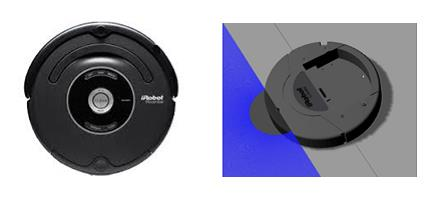
\includegraphics[width=0.85\textwidth, height=5.5cm]{figures/roomba.jpg}
		\caption{Modelo Roomba}
		\label{fig.roomba}
		\end{center}
\end{figure}

Para poder acceder a la funcionalidad que ofrece, se han utilizado tres \textit{plugins} que ejercen de drivers de la aspiradora:

\begin{itemize}
	\item \textit{pose3di}: Los componentes harán uso de este \textit{plugin} para obtener su posición en tiempo real, sólo se empleará la odometría.
	\item \textit{motorsi}: Este \textit{plugin} interactúa con el componente, dotándole de velocidad, ya sea velocidad de tracción o de rotación.
	\item \textit{Laseri}: Este \textit{plugin} será usado por los componentes para obtener información de la distancia entre él y los obstáculos dentro de un sector. 
\end{itemize}

Cabe mencionar en este punto que este robot no ha sido el único modelo empleado. En vistas a añadir mejoras a la práctica, se detallará en \textbf{5.4} el empleo de interfaces \textit{ROS Messages} para la interacción con el robot, para lo cual se ha utilizado una combinación de modelos que incluye el paquete \textit{ros-kinetic} basada en la versión americana de \textit{Roomba}, el robot \textit{Create}, y un modelo conocido de sensor láser como es \textit{Hokuyo}. Reservamos el resto de información relevante para dicho apartado, ya que la solución principal empleará el robot \textit{Roomba}.

\subsubsection{Sensor láser}
En la parte frontal del robot se ha modelado un sensor láser que se utilizará en todo momento en la práctica, por lo que constituye el sensor más importante a estos efectos. 

Está compuesto por un \textit{array} de 180 medidas, que puede medir distancia alrededor de 180 grados en milímetros, con precisión de 1 grado. Su funcionamiento se basa en emitir rayos láser en todas estas orientaciones, que rebotan sobre los objetos existentes (si los hay) de manera no especular, de tal manera que al recibir el rayo devuelto se calcula la distancia al objeto según el tiempo de vuelo.

Una vez más la plataforma JdeRobot encapsula la complejidad de este sensor y su API de utilización. Únicamente se ha construido un \textit{parser} para la práctica que agrupa los datos en forma de \textit{array} de 180 distancias, donde el índice es el ángulo de proyección del haz del láser.
 
\subsubsection{Sensor Odométrico}
En ésta práctica jugará un papel importante el saber cuánto se ha desplazado el robot en un intervalo, dado que servirá para desechar o evolucionar datos involucrados en el algoritmo de auto-localización que explicaremos en \textbf{5.5.1}. Ésta es precisamente la función de la odometría: el uso de sensores de movimiento para determinar el cambio de posición del robot en relación con una posición conocida. Si el robot conoce el diámetro de sus ruedas, simplemente le basta con contar el número de revoluciones de las mismas para determinar qué tan lejos ha viajado. Normalmente, el conteo de vueltas se realiza a través de \textit{encoders}, que emiten un número fijo de pulsos por revolución, siendo éstos los registrados por el software.

Así, el sentido de giro y el número de vueltas que da cada rueda nos ayudará a saber en qué dirección se ha movido el robot, y cuánta distancia ha recorrido.

\subsection{Modelo Asymmetric-Easy-To-Model} 
Dado que la aspiradora necesita un entorno acotado para poder determinar su localización (el láser tiene un alcance limitado), ha sido necesario crear un modelo para que la aspiradora navegue en ella.
Hemos partido del diseño \textit{house\_int2} que utiliza la práctica \textit{Vacuum Cleaner} de JdeRobot-Academy como punto de partida. Este modelo se puede ver en la \textbf{Figura 5.2}:

\begin{figure}[H]
  \begin{center}
    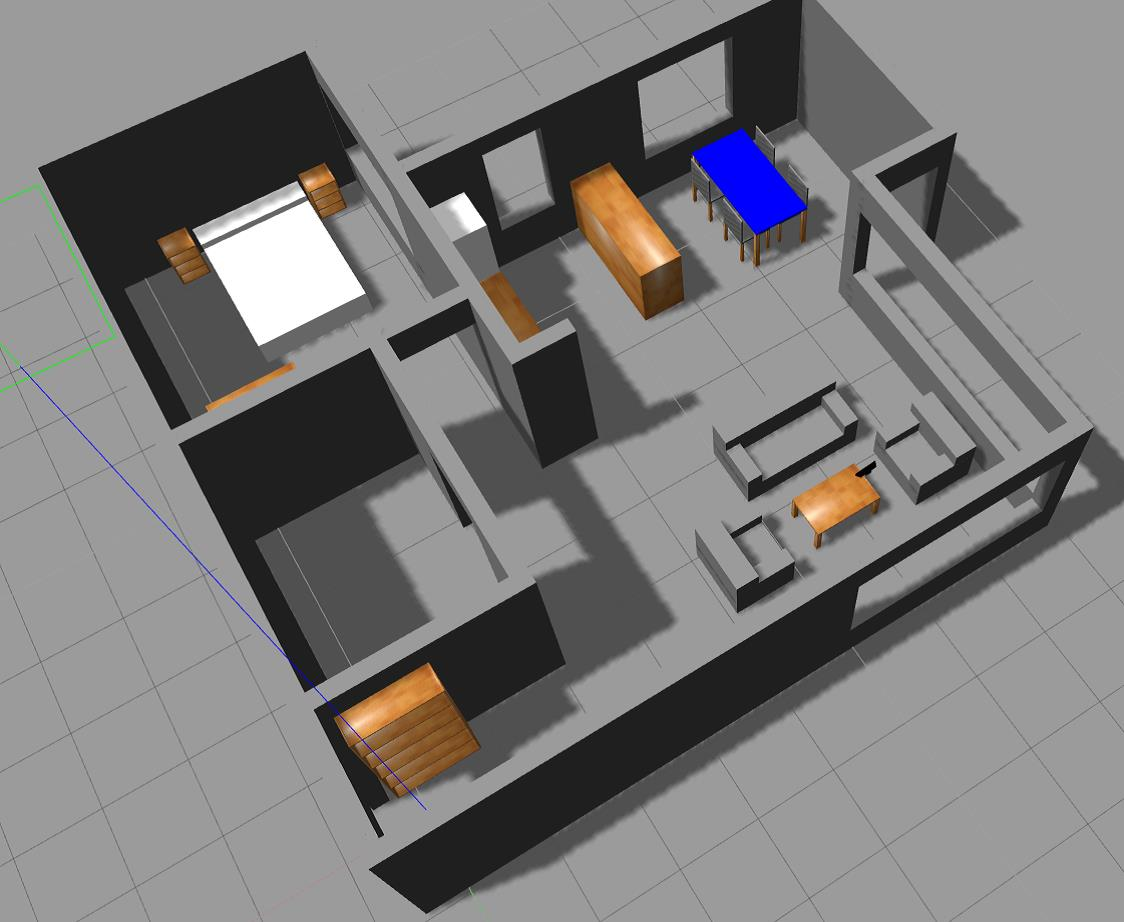
\includegraphics[width=0.75\textwidth]{figures/houseint.jpg}
		\caption{Modelo house\_int2}
		\label{fig.houseint}
		\end{center}
\end{figure}

Las razones bajo la elección de este modelo son:

\begin{itemize}
	\item[--] Entorno acotado por paredes, ideal para obtener lecturas del sensor láser representativas.
	\item[--]	Abundantes obstáculos, lo cual favorece la diferencia entre lecturas en cada punto de la casa.
	\item[--]	Malla de colisiones bien definida, importante cuando se quiere que el robot navegue por la casa sin la aparición de sucesos extraños, como objetos voladores al colisionar con ellos. 
\end{itemize}

Aún con todo ello, este modelo emplea elementos de difícil modelado en una imagen 2D (necesaria para establecer el mapa del mundo), como puede ser la mesa y las sillas: cada pata debía tener el tamaño exacto a escala y estar en la posición adecuada para no obtener procesados erróneos. La zona bajo la cama también resultó un problema. 

Dadas las múltiples ventajas que presenta, se ha creado un nuevo modelo, basado en el anterior, que sustituye todos los elementos difíciles de modelar por paredes, claramente definidas y representadas, mucho más fáciles de modelas en una imagen. Al nuevo mundo que incluía este modelo y el modelo de aspiradora se le ha llamado \textit{Asymmetric-Easy-To-Model.world} (\textbf{Figura 5.3}):

\begin{figure}[H]
  \begin{center}
    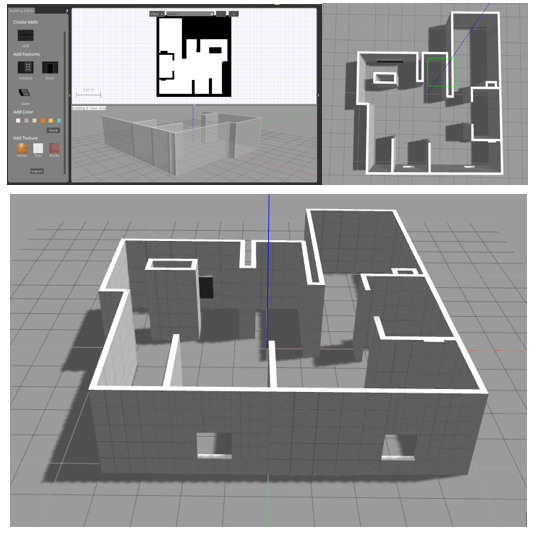
\includegraphics[width=0.95\textwidth, height=12cm]{figures/modeloasymmetric.png}
		\caption{Modelo Asymmetric-Easy-To-Model}
		\label{fig.modeloasymmetric}
		\end{center}
\end{figure}

Como se puede ver, el mundo conserva su forma asimétrica (distintas formas son observadas por el robot en cada orientación y posición) pero está caracterizado por un modelado mucho más simple. 

\subsection{Modelo Choso}
El modelo anterior es el caso más común en el que nos encontramos con el problema de la auto-localización, dada la naturaleza asimétrica del entorno que nos rodea. No obstante, también existen lugares no tan cambiantes, donde las formas se repiten o las superficies límite son iguales o similares en distintas orientaciones. Es por eso que hemos decidido crear el mundo de Gazebo \textit{Choso.world}, el cual es una habitación cuadrada con sólo dos elementos, que ocupan muy poco espacio y por tanto pasan desapercibidos en la mayoría de casos. Este modelo se puede ver en la siguiente imagen (\textbf{Figura 5.4}):

\begin{figure}[H]
  \begin{center}
    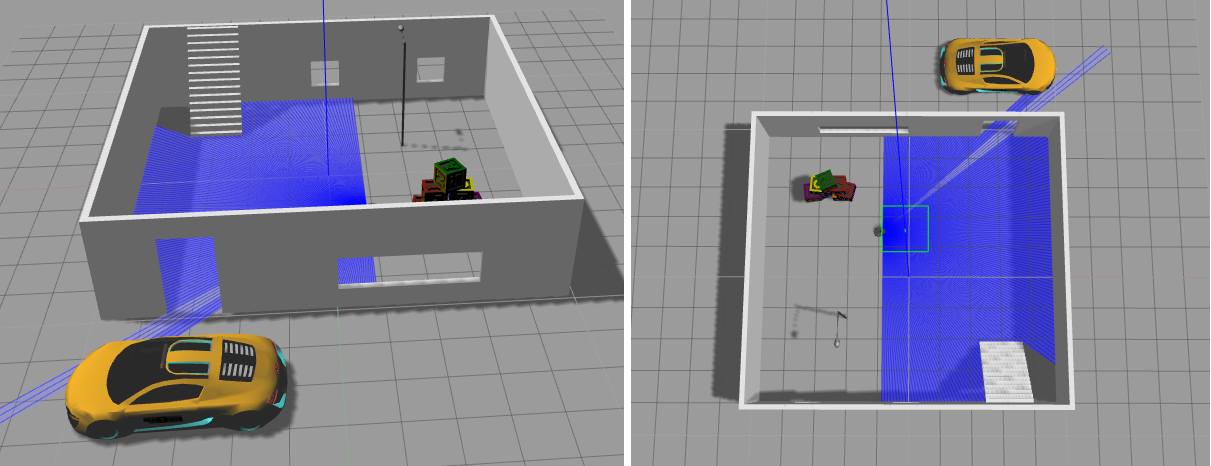
\includegraphics[width=0.96\textwidth]{figures/chosoworld.png}
		\caption{Modelo Choso}
		\label{fig.choso}
		\end{center}
\end{figure}

Introduciremos al robot en este modelo creando un mundo simétrico con fines de experimentación y verificación del comportamiento del algoritmo.

\subsection{Mundo de Gazebo}
A partir de este punto, y a no ser que se indique explícitamente lo contrario, cuando se hable del mundo empleado se asumirá que el modelo empleado es \textit{Asymmetric-Easy-To-Model}.

Así, incorporando los dos modelos involucrados (\textit{Asymmetric-Easy-To-Model} y \textit{Roomba}) y algunas fuentes de luz como el sol, luz ambiente y algunas sombras, se crea el mundo principal en el que abordar la práctica: \textit{Asymmetric-Easy-To-Model.world}(\textbf{Figura 5.5}). Debido a la extensión del fichero de descripción del mundo, sólo incluimos a continuación una parte del mismo para observar su aspecto:

\begin{figure}[H]
  \begin{center}
    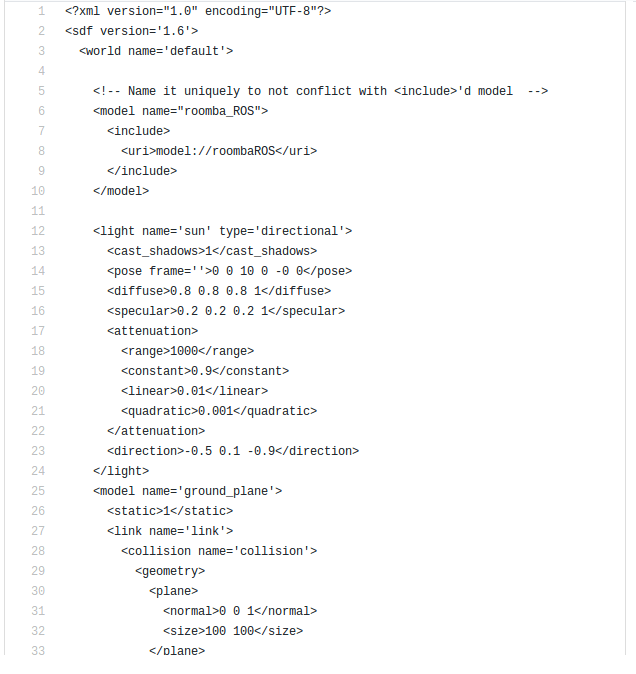
\includegraphics[width=0.98\textwidth]{figures/codeworld.png}
		\caption{Código del mundo}
		\label{fig.codeworld}
		\end{center}
\end{figure}

En él, se puede ver la combinación del modelo re robot creado y de los parámetros de física, aspecto, iluminación y posición que componen el mundo.

\section{Componente Académico}
El componente académico que se ha preparado para esta práctica recoge toda la funcionalidad para ayudar al alumno a enfrentarse a ella y resolverla con éxito. Estas son las piezas que conforman el componente y que quedan resueltas a través de él:  

\begin{enumerate}[label=\alph*)]
	\item Ofrece una interfaz gráfica al usuario que le ayuda a depurar su código; 
	\item Ofrece acceso a todas las interfaces que el robot posee, tanto sensores como actuadores, en forma de métodos simples (oculta el \textit{middleware} de comunicaciones); 
	\item Incluye código auxiliar, como \textit{parsers} o constructores de objetos, que no son parte del algoritmo a realizar, sino que sólo sirven de ayuda para hacer la tarea algo más sencilla.
\end{enumerate}

El componente pone la base que el estudiante culmina incluyendo su código en el método \textit{execute} del fichero \textit{MyAlgorithm.py}, siempre realizando las pruebas que considere oportuno para pulir su solución.

El nodo ofrece un API de sensores y actuadores al programador, además de un API específico para la práctica en el que se encontrarán otros métodos e incluso variables disponibles para facilitar la tarea. En cuanto al API del robot, tenemos:

\begin{itemize}
	\item \textit{self.sensors.motors.sendVelocities(vel)}: Para enviar comandos de velocidad a través de:
    \begin{itemize}[label={$\diamond$}]
			\item \textit{vel = CMDVel()}: constructor de comandos de velocidad
       \item \textit{vel.vx = valor}: velocidad lineal
       \item \textit{vel.az = valor}: velocidad angular
    \end{itemize}
    \item \textit{self.sensors.laserdata} o \textit{self.gui.getLaserData()}: dos posibilidades equivalentes para obtener los datos láser.
    \item \textit{self.parse\_laser\_data(laser)}: Para transformar los datos láser en una estructura más fácilmente manejable.
		\item \textit{self.pose3d.getPose3d().x}, \textit{self.pose3d.getPose3d().y}, \textit{self.pose3d.getPose3d().yaw}: para obtener los datos de posición y orientación del robot.
\end{itemize}

Por otro lado, la manera de utilizar la funcionalidad que este nodo ofrece resuelta es:

\begin{itemize}
	\item ||\textbf{Clase Particle}||: \textit{Particle(x, y, yaw, prob, self.map.robotAngle)}: Constructor de partículas.
	\item \textit{self.setParticles([p1,p2,p3,...])}: Representa una lista de partículas en el GUI.
	\item \textit{self.setEstimation(particle)}: Para mostrar una estimación en el interfaz
	\item \textit{img = self.map.pixmap.toImage()}: para obtener la imagen (mapa) del interfaz.
	\item \textit{self.paintTheoricalLaser(theoricalLaser)}: para representar un láser en la interfaz.
	\item \textbf{(variable)} \textit{self.particleClicked}: almacena la última partícula sobra la que se ha hecho click en el GUI. 
	\item \textit{self.map.map2pixel((x,y))}: obtiene el pixel correspondiente a las coordenadas (x,y).
	\item \textit{self.map.pixel2map((px,py)}: obtiene las coordenadas reales asociadas al pixel [px,py] del mapa.
\end{itemize}

Con ello, todo lo necesario queda a disposición del alumno para comenzar la tarea. El único componente externo que el nodo académico necesita es un fichero de configuración que recoja los \textit{endpoints} que las interfaces de los sensores y actuadores descritos en \textbf{5.2.1}, \textbf{5.2.1.1} y \textbf{5.2.1.2} utilizan para publicar la información o recibirla del nodo. Este archivo tiene extensión \textit{.yml}, lo cual implica que debe cumplir las especificaciones del formato de serialización de datos YAML. Para esta práctica en concreto, añadimos además la configuración necesaria para establecer el mapa binario de referencia del robot. Tiene el siguiente aspecto(\textbf{Figura 5.6}):

\begin{figure}[H]
  \begin{center}
    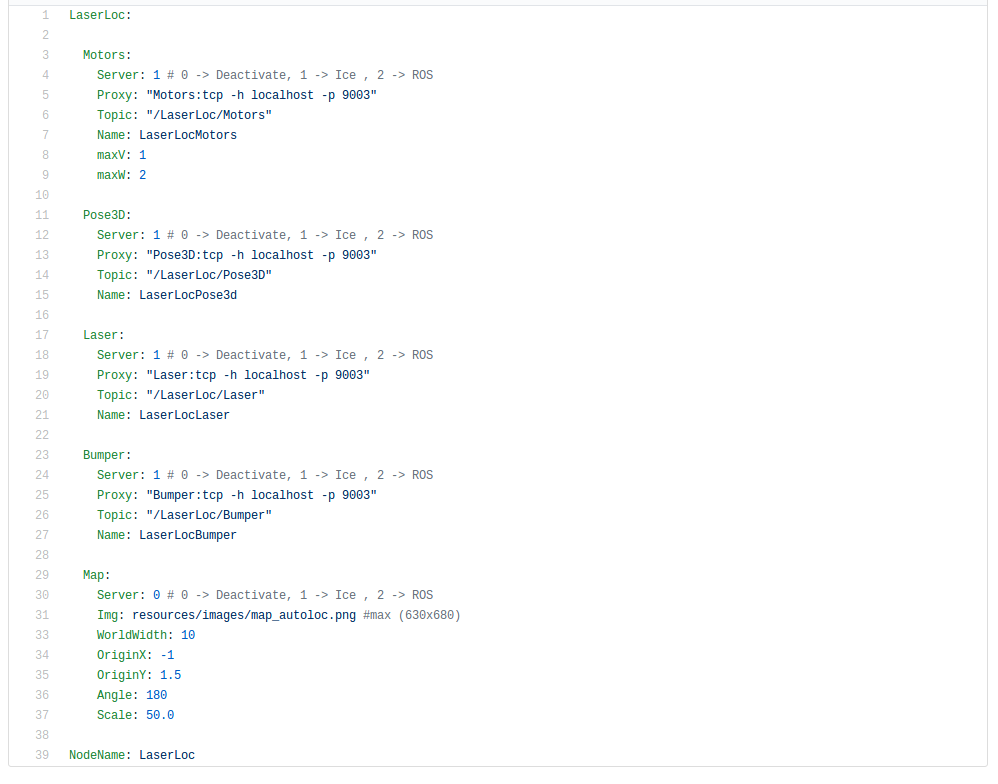
\includegraphics[width=0.98\textwidth]{figures/ymlantiguo.png}
		\caption{Fichero de configuración YAML de LaserLoc}
		\label{fig.llyaml}
		\end{center}
\end{figure}

En la versión básica, todas las comunicaciones se realizarán a través de ICE, a falta de \textit{plugins} que administren los sensores y actuadores a través de \textit{ROS Messages}. Otra versión de la práctica utilizando estos interfaces será descrita en \textbf{5.4}, demostrando que JdeRobot es totalmente compatible con ROS, únicamente retocando en este fichero de configuración el \textit{flag} que indica si el servidor de datos es uno u otro. Además, vemos que la información del mapa cuenta con atributos como el tamaño, la escala o el \textit{path} que conduce a la imagen binaria. Por último, se establecen las velocidades máximas de tracción y rotación en base a las necesidades de la práctica. Cabe mencionar que gracias a la configuración interna de la plataforma JdeRobot es posible que las distintas interfaces utilicen un mismo puerto.

El componente se ha segmentado en distintos hilos para favorecer la simultaneidad de ejecución de distintas tareas clave. En un principio, el componente sólo contaba con dos hilos básicos de ejecución:

\begin{itemize}
  \renewcommand{\labelitemi}{$\to$}
	\item Hilo de algoritmo: se encarga del refresco de la ejecución del algoritmo, ya que este se ejecuta de modo iterativo o cíclico. El tiempo de refresco es importante, dado que el algoritmo necesario para solventar la práctica es bastante sensible a pequeños cambios en las lecturas, que deben desencadenar correcciones en la ejecución. Por ello, el tiempo de refresco es de 10 ms.
	\item Hilo de la interfaz gráfica de usuario (GUI): Este hilo es el encargado de actualizar la interfaz gráfica y los \textit{widgets} incorporados en ella. El intervalo de actualización de la interfaz debe ser pequeño, de tal manera que los cambios en los sensores o en el mapa puedan ser representados en tiempo real. Por ello, se ha fijado el tiempo de refresco a 20 ms.
\end{itemize}

Estos agilizaban la respuesta de los distintos módulos implicados. Sin embargo, se hizo necesario añadir un tercer hilo de ejecución:

\begin{itemize}
  \renewcommand{\labelitemi}{$\to$}
	\item Hilo de sensores: el tercer hilo se ha añadido para actualizar los datos de los sensores y los actuadores a través de las interfaces que correspondan (ICE o ROS). El tiempo de refresco de este hilo es muy importante, dado que un intervalo largo radicaría en lecturas desactualizadas de los sensores. Por ello, dicho tiempo también se ha fijado en 20 ms.
\end{itemize}

Esto se debe a la sobrecarga aritmética que el algoritmo de localización introduce en el componente. Entraremos más en detalle sobre esta decisión en \textbf{5.5.2}.

Con todo ello, el nodo dispone la interfaz de usuario con algunos elementos de depuración (accesibles a través del API descrito más arriba) para que el usuario se centre en el algoritmo a escribir. La manera de integrar dicho algoritmo en el nodo para que llegue al robot también es tarea del componente académico, por lo cual se reserva un espacio concreto para que el alumno inserte la lógica, debidamente indicado en el fichero de instrucciones incluido (\textit{README.md}).

\subsection{Interfaz gráfica}
La interfaz gráfica de usuario (GUI) se emplea para representar información que pueda ayudar a resolver el algoritmo planteado, lo cual resultará vital en el camino hacia la resolución de la misma. Se ha construido a través de PyQt5, y se encargará de mostrar la salida de la ejecución del algoritmo en cada instante, ideal para depurar y observar su evolución.

\begin{figure}[H]
  \begin{center}
    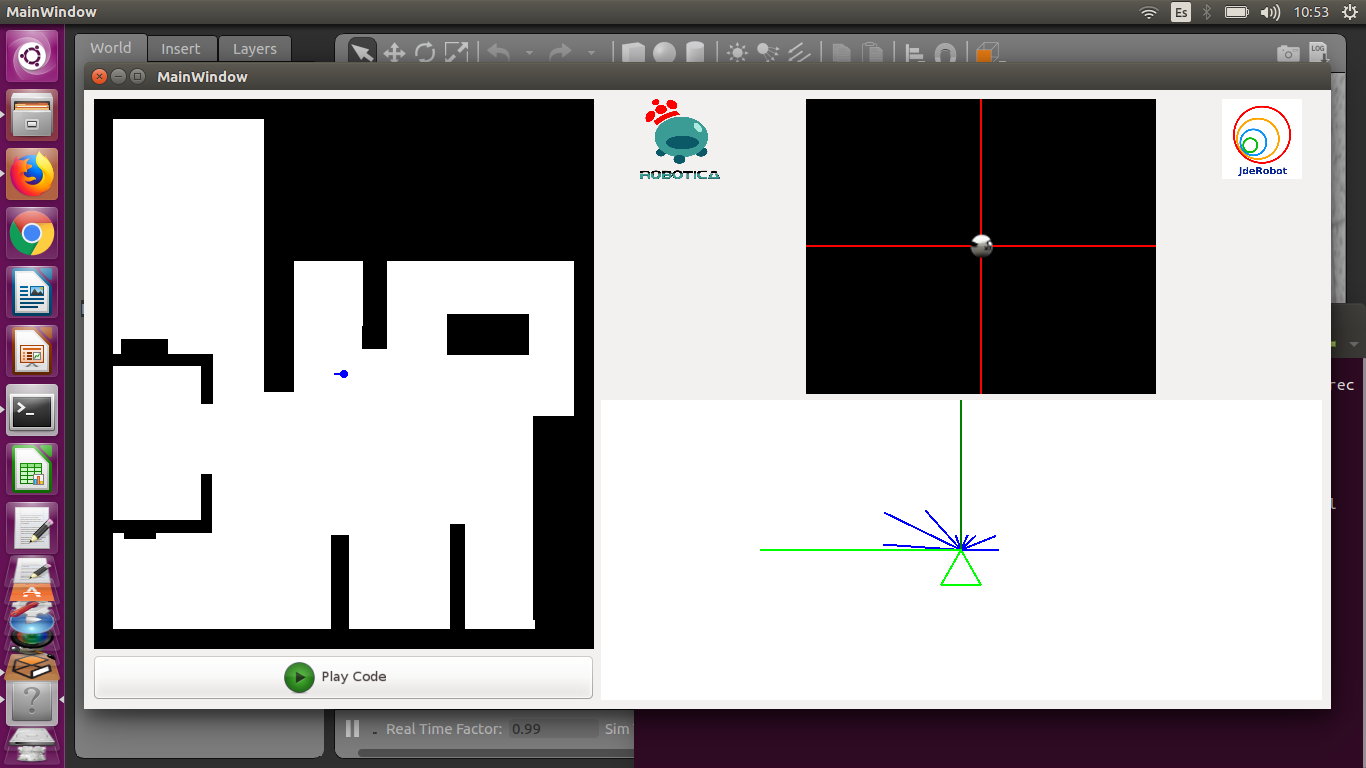
\includegraphics[width=0.98\textwidth]{figures/llgui.png}
		\caption{Interfaz Gráfica Laser Loc}
		\label{fig.llgui}
		\end{center}
\end{figure}

Esta GUI (\textbf{Figura 5.7}) está formada por 3 \textit{widgets} para el control y visionado del comportamiento del robot. El primero de ellos, situado a la izquierda, es quizás el más importante, pues muestra al programador un mapa binario que el robot utiliza para poder realizar cálculos pertinentes para llevar a cabo su auto-localización, pero con información gráfica con la que este no cuenta: las sucesivas generaciones de partículas (información ampliada en \textbf{5.3.3.1}) que surgen del algoritmo evolutivo que se ha de usar, el cual comentaremos en \textbf{5.5}. Así, en el mapa se ven reflejados los obstáculos (zonas negras), las zonas libres (espacio en blanco), la posición y orientación del robot en el espacio dado (a través de un punto azul), la evolución de las partículas e incluso las trayectorias (ver \textbf{5.3.3} para más detalles). 
El segundo de los elementos del interfaz, situado en la parte superior derecha es el clásico teleoperador, el cual se incorpora en todas las prácticas para añadir la capacidad de controlar la posición del robot y su rotación a través de órdenes de velocidad lineal y angular. Esto facilita el proceso de depuración y sirve de apoyo en los primeros pasos hacia la solución.

Por último, el espacio inferior derecho se ha reservado para la representación de las lecturas que ofrece el láser del robot en cada momento, y también para graficar de manera aproximada el cálculo de láser teórico que el robot hace de cada partícula (ver \textbf{5.3.2}).

En la parte inferior se ha incluido un botón para ejecutar el algoritmo y pararlo cuando sea necesario, lo cual también para todas las representaciones y el movimiento del robot. 

\subsection{Gráfica de los láseres Real y Teórico}
Como se ha comentado en el punto anterior, uno de los elementos de visualización que incluye la práctica es la posibilidad de ver de forma gráfica los datos que ofrece el sensor láser, así como una representación de los haces láser de cada partícula calculados a partir de la lectura que ofrecería el robot en el caso de que su posición y orientación coincidiesen con los de esta. Así, lo que se representa es lo siguiente:

\begin{enumerate}
	\item \textbf{- Láser Real}
	\begin{figure}[H]
		\begin{center}
			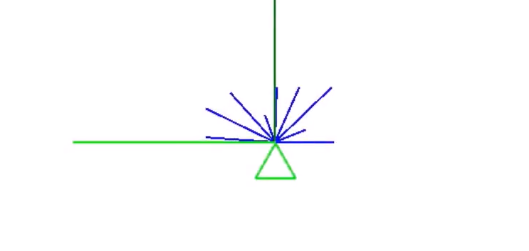
\includegraphics[width=0.65\textwidth]{figures/laserreal.png}
			\caption{Laser Real}
			\label{fig.laserreal}
			\end{center}
	\end{figure}
Dado que las lecturas utilizadas para esta práctica están formadas por 9 haces en total (uno cada 20º con respecto a la normal de la orientación del robot), lo que se representa es un conjunto de segmentos cuya longitud se corresponde con la distancia (a escala 50:1) al primer obstáculo en la dirección marcada por el ángulo del haz (\textbf{Figura 5.8}). Como se dijo en \textbf{5.2.1.1}¸ las medidas del láser constan de 180 pares de valores, y su reducción a los 9 utilizados se describirá en \textbf{5.5.2}. Los datos de \textit{parsean} convenientemente antes de ser representados, y la representación es en todo caso absoluta (no tiene en cuenta la orientación del robot, ya que en caso contrario la resolución de la práctica sería una tarea mucho más sencilla).
\item \textbf{- Láser Teórico}
	\begin{figure}[H]
		\begin{center}
			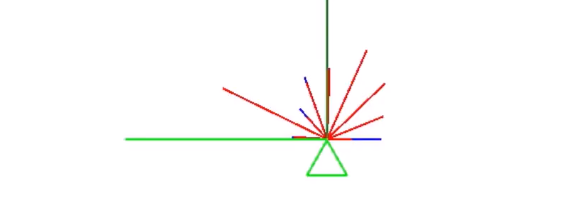
\includegraphics[width=0.65\textwidth]{figures/laserteorico.png}
			\caption{Laser Teórico}
			\label{fig.laserteorico}
			\end{center}
	\end{figure}
Como veremos más adelante, para cada partícula involucrada en el algoritmo se deberá calcular un “láser teórico” (\textbf{Figura 5.9}), nombre con el que hemos bautizado a la lectura que se obtendría en el sensor en el supuesto de que el robot ocupase la posición de dicha partícula y compartiese su orientación. Se puede ver que en la representación se muestra la superposición de ambos datos láser: el real en azul y el teórico en rojo, de manera que en todo momento se puede comprobar si una partícula ofrece una lectura similar a la del robot o no. Dado que el algoritmo se compone de muchas partículas, para activar la representación del láser teórico de una partícula determinada bastará con hacer click sobre ella en el \textit{widget} que contiene el mapa de referencia. De nuevo, la representación es absoluta, no relativa a las características de cada partícula.
\end{enumerate}

\subsection{Mapa de Referencia}
El elemento gráfico vital es el mapa que robot utiliza para poder hacer cálculos sobre su entorno. Este mapa es una imagen con sólo dos valores posibles para cada pixel: blanco y negro. Esto facilita las tareas de procesado, ya que se tiene un juego de valores fijo, reducido y conocido. El robot se va a basar en dicho mapa para poder realizar el cálculo de los datos teóricos láser, llevando a cabo un método de trazado de rayos sobre la imagen sobre el que se profundizará en la explicación de la solución. Este mapa emplea una codificación de color para expresar visualmente la probabilidad de cada suceso, como el que se muestra en la \textbf{Figura 5.10}.

\begin{multicols}{2}
\begin{figure}[H]
		\begin{center}
			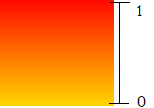
\includegraphics[width=0.3\textwidth]{figures/gradcolor.png}
			\caption{Codificación de color}
			\label{fig.gradcolor}
			\end{center}
	\end{figure}

Así, cada partícula se representará con un color dentro de este rango, en función de sus posibilidades de ser la posición real en la que se encuentra el robot.

Hay dos excepciones para esta codificación de color:
\end{multicols} 

\begin{itemize}
	\item[--] La posición real del robot, también representada en forma de partícula, utilizará un color azul oscuro en todo momento
	\item[--] Las estimaciones que el robot hará de su posición se representarán en azul claro.
\end{itemize}

Por último, este lienzo también superpondrá al mapa la trayectoria que el robot sigue en todo momento representada en negro, y la trayectoria estimada por el robot para localización en movimiento, representada también en azul claro, como se ve en la \textbf{Figura 5.11}:

\begin{figure}[H]
	\begin{center}
		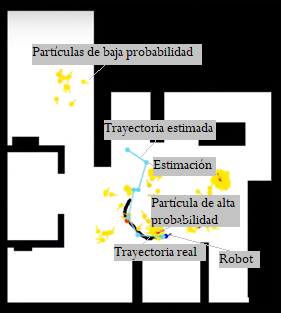
\includegraphics[width=0.5\textwidth]{figures/mapareferencia.png}
		\caption{Mapa de referencia}
		\label{fig.mapareferencia}
		\end{center}
\end{figure}

\subsubsection{Partículas}
El elemento principal en el que se basa el algoritmo que se debe emplear en la solución son las partículas, las cuales ya hemos mencionado en el desarrollo de este capítulo. Lo primero es explicar su composición y características:

Estas partículas no son más que puntos en el espacio en los que el robot se proyecta a sí mismo, es decir, posiciones y orientaciones que el robot puede ocupar y tomar en el escenario. Por ello, cada partícula consta de:

\begin{itemize}
  \renewcommand{\labelitemi}{$\to$}
	\item Un vector de coordenadas (x, y, z) que representa su posición en el espacio. Todas las posiciones ocupadas por algún obstáculo no están disponibles para el robot, de manera que tampoco pueden estarlo para las partículas. La coordenada z se fija siempre a 0, dado que el escenario no contiene desniveles.
	\item Un atributo de orientación, que representa su rotación con respecto al mapa. 
	\item Un valor de probabilidad, que almacena el valor numérico obtenido al comparar el láser de la partícula con la lectura real.
\end{itemize}

A fin de organizar el código, se ofrece al programador la clase \textit{Particle}¸ la cual actúa como constructor de partículas, asociando a cada una sus correspondientes características accesibles como atributos de un objeto Python:

\begin{figure}[H]
	\begin{center}
		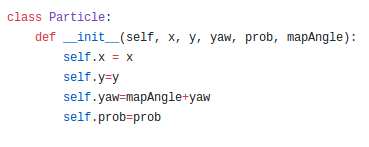
\includegraphics[width=0.6\textwidth]{figures/claseparticle.png}
		\label{fig.claseparticle}
		\end{center}
\end{figure}

\subsubsection{Trayectorias}
En cuanto a las trayectorias que se representan en el gráfico, cabe decir que la ruta real está formada por las últimas 100 posiciones diferentes que ha ocupado el robot para su representación, de manera que se modifica con las sucesivas iteraciones. Sirve como apoyo para pulir el comportamiento del algoritmo, ya que el programador podrá compararla en todo momento con la trayectoria que su lógica implementada va creando. Su representación es automática y se encarga la interfaz del nodo académico.

Por otro lado, la trayectoria estimada es obtenida a través de la unión de las distintas estimaciones de posición que el algoritmo del robot hace a lo largo del tiempo. Se ha dotado al componente con un API para el establecimiento de estimaciones a visualizar en la gráfica:

\hspace{0.32\linewidth} \textit{self.setEstimation([x,y])}

Con lo cual se puede hacer un seguimiento del comportamiento del algoritmo a largo plazo.
 
\section{Comunicaciones con ROS}
A fin de crear la primera práctica auto-contenida del entorno JdeRobot, se utilizará interfaces de ROS para implementar una nueva versión de la práctica que no dependa del paquete de comunicaciones que emplean todas las prácticas de Academy (\textit{JdeRobotComm}), de tal manera que un supuesto usuario futuro sólo tendría que instalar en su máquina el simulador, el paquete \textit{kinetic} de ROS y los interfaces y \textit{plugins} necesarios y los modelos y mundos preparados por el entorno. Con esto, sólo se habría de clonar el repositorio del entorno académico en el cual están las prácticas y empezar a programar, sin la necesidad de instalar otros paquetes necesarios para ejecutar las prácticas actuales del entorno. Dado que ROS tiene soporte en distintas plataformas, se conseguiría tener una práctica totalmente funcional para muchos usuarios diferentes.

\begin{multicols}{2}
	\begin{figure}[H]
	\begin{center}
		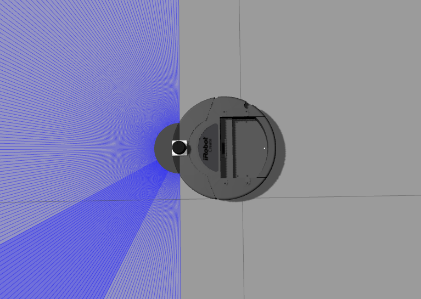
\includegraphics[width=0.3\textwidth]{figures/create.png}
		\caption{Modelo Roomba ROS}
		\label{fig.create}
		\end{center}
\end{figure}

El nuevo robot (\textbf{Figura 5.12}) conserva todas las interfaces de sensores y actuadores anteriores (incluidas aquellas no utilizadas en esta práctica como el \textit{bumper}), por lo que su funcionalidad es equivalente.
\end{multicols}
En cuanto al sensor láser, hemos utilizado un modelo ya creado llamado \textit{hokuyo} (\textbf{Figura 5.13}) que ya se comunica a través de \textit{ROS Messages}, el cual se ha incrustado en la parte frontal del robot.

Para conservar la funcionalidad que ofrecía la aspiradora en la simulación, hemos usado los siguientes \textit{plugins}:

\begin{multicols}{2}
	\begin{figure}[H]
	\begin{center}
		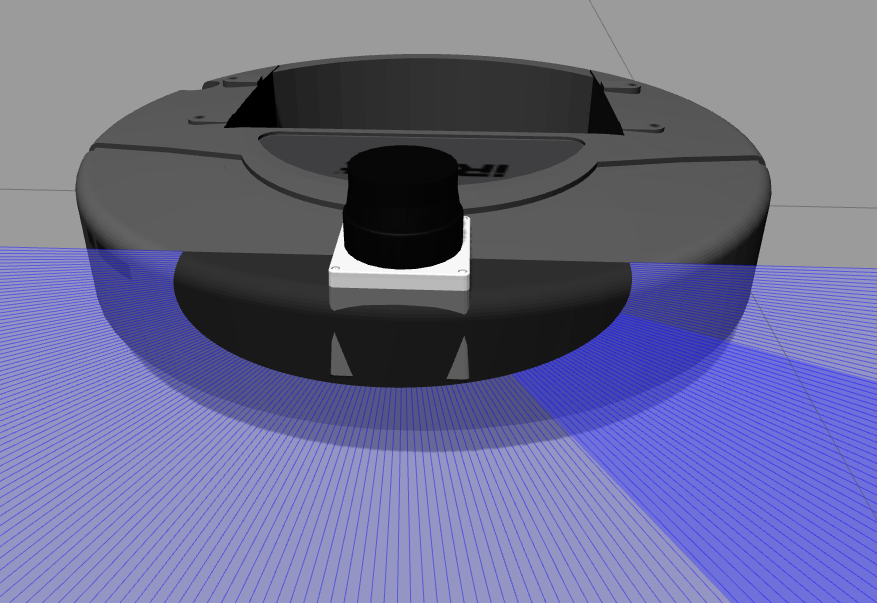
\includegraphics[width=0.3\textwidth]{figures/hokuyo.png}
		\caption{Modelo Hokuyo sobre Roomba}
		\label{fig.hokuyo}
		\end{center}
\end{figure}

\begin{itemize}
	\item \textit{libgazebo\_ros\_bumper.so} 
Para gestionar el sensor bumper
	\item \textit{libgazebo\_ros\_laser.so}  
Para recibir datos del sensor láser
	\item \textit{libgazebo\_ros\_diff\_drive.so } 
Para obtener odometría y controlar motores
\end{itemize}
\end{multicols}

Todos ellos compatibles con la versión \textit{kinetic} de ROS.

Una vez creado el modelo, basta con incluirlo en el mundo del que ya disponíamos para poder usarlo. No obstante, son necesarios unos pequeños cambios en el nodo:

Como ya hemos dicho, perseguíamos una práctica auto-contenida, de manera que el fichero principal del nodo (\textit{laser\_loc.py}) debe ahora incluir todo lo necesario para establecer y mantener la comunicación con el robot, y para realizar la conversión entre los mensajes recibidos y los datos que el nodo puede manejar. 

Por tanto, dicho fichero debe contener:
\begin{enumerate}
	\item El código necesario para conectar con cada nodo del robot, para lo cual se usan sentencias tipo:
	\begin{figure}[H]
	\begin{center}
		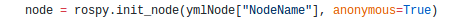
\includegraphics[width=0.75\textwidth]{figures/initnode.png}
		\label{fig.initnode}
		\end{center}
	\end{figure}
	\item La suscripción de cada nodo inicializado a su correspondiente \textit{topic} de ROS, es decir, a su bus de intercambio de mensajes en el cual el driver encargado del control del nodo (ya sea sensor o actuador) publica o recibe mensajes con cierta forma:
	\begin{figure}[H]
	\begin{center}
		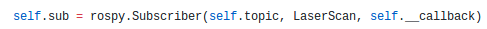
\includegraphics[width=0.75\textwidth]{figures/subscriberlaser.png}
		\label{fig.subscriberlaser}
		\end{center}
	\end{figure}
	\hspace{0.48\linewidth}o
	\begin{figure}[H]
	\begin{center}
		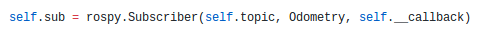
\includegraphics[width=0.75\textwidth]{figures/subscriberodometry.png}
		\label{fig.subscriberodometry}
		\end{center}
	\end{figure}
	\item La transformación de los mensajes que se intercambian por los buses y la utilizada por el nodo de la práctica:
	\begin{figure}[H]
	\begin{center}
		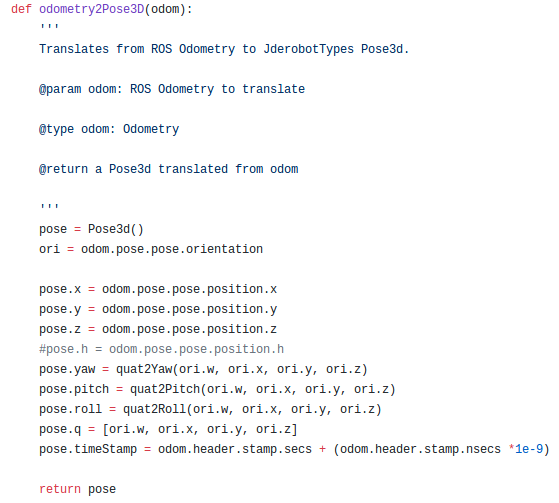
\includegraphics[width=0.60\textwidth]{figures/odom2pose.png}
		\label{fig.odometry2pose}
		\end{center}
	\end{figure}
\end{enumerate}

Para todo ello, el nuevo fichero principal amplía su funcionalidad con una serie de clases que se encargan de la construcción de objetos que tengan en cuenta todas las especificaciones anteriores.
La asociación entre cada nodo y su \textit{topic} se traduce en una serie de cambios en el fichero de configuración (\textbf{Figura 5.14}) que se facilita a la hora de ejecutar:

\begin{figure}[H]
	\begin{center}
		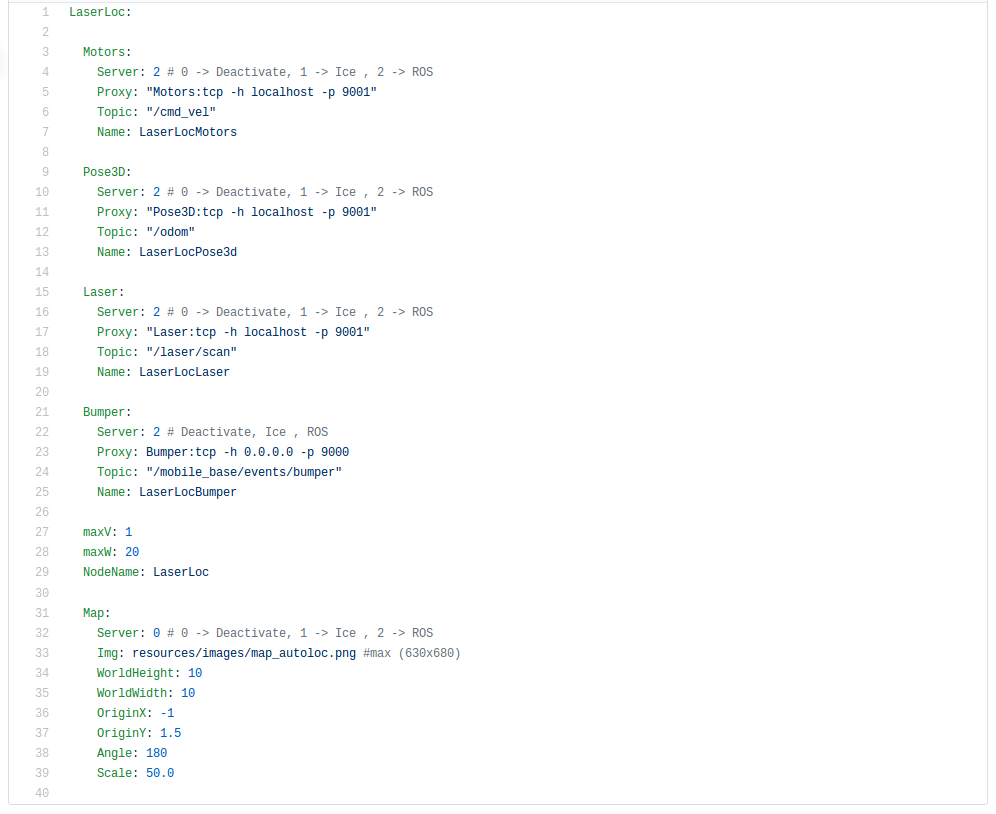
\includegraphics[width=0.98\textwidth]{figures/llymlfinal.png}
		\caption{Fichero de configuración YAML con interfaces de ROS}
		\label{fig.llymlfinal}
		\end{center}
\end{figure}

Por lo demás, y al estar hecho de manera genérica, no son necesarios más cambios en ningún otro componente del nodo gracias a la compatibilidad de JdeRobot con el \textit{middleware}.

\section{Solución de referencia}
Persiguiendo el objetivo de implementar la lógica de auto-localización del robot de esta práctica, la solución ha de contener un algoritmo de procesado de imagen combinado con un algoritmo matemático que permita implementar el filtro de partículas. Para esta práctica no es adecuado incluir también un algoritmo de pilotaje, pues a estos efectos se dispone de un teleoperador, lo que contribuirá a que la ruta seguida por el robot sea en todo caso aleatoria, permitiendo así comprobar las prestaciones del algoritmo reactivo resultante de manera más crítica. 
Comenzaremos esta sección describiendo los distintos tipos de algoritmos de localización existentes, argumentando el porqué del que hemos escogido. Con ello construiremos una solución que se establecerá como solución de referencia en la plataforma, pero que sólo es uno de los muchos posibles métodos con el cual alcanzar el fin. El código quedara recogido en el fichero \textit{MyAlgorithm.py} que para este caso también tiene naturaleza iterativa, de manera que en cada iteración se obtiene datos de los sensores, se procesa y se actúa en consecuencia (se evoluciona el algoritmo). El código a escribir irá de nuevo a parar al método \textit{execute}, el cual debe ejecuta la lógica de manera cíclica en el \textit{thread} de algoritmo y computación.

\subsection{Algoritmos de autolocalización}
El campo de la localización se puede dividir en dos grandes subgrupos: el primero y más sencillo es partir de una posición inicial conocida, en este caso para determinar la posición final del robot habrá que estimar los errores acumulados por los odómetros. El segundo y más difícil aborda lo que se conoce como localización global, en la que se desconoce la posición inicial del robot y los errores son mayores que en el caso anterior, ya que en este caso hay más fuentes que los introducen. Nosotros pretendemos abordar precisamente este segundo caso, para el cual hay que tener en cuenta varios parámetros cambiantes que a su vez hacen que cambien el problema y la solución.
Es por eso que las distintas maneras de abordar el problema se gradúan en base a su dificultad, dependiendo por ejemplo en el tipo de láser utilizado, ya que emplear sensores de posición facilita en gran medida la localización (como mucho habrá que estimar y corregir los errores o derivas del sensor) u otros equivalentes como sensores GPS (en exteriores) o localización geométrica a través de balizas. Sin embargo, la versión más difícil y elaborada del problema de la localización, es enfrentarse a ella usando sensores no específicos de posición (láser, cámaras,..). En este caso la información de posición se obtiene relacionando las lecturas sensoriales con el mapa del entorno.
Existen diferentes técnicas como el \textit{scan maching} que se basa en ir “superponiendo” lecturas del mapa local sobre el global intentado ajustar las lecturas a este último, pero no es apta para localización global. Otra técnica buena para la localización local son los filtros de Kalman, un filtro de Bayes recursivo que estima la distribución a posteriori del estado de un sistema condicionada en función de los datos. Su principal limitación es que se trata de una técnica unimodal y exclusivamente gaussiana [Isard y Blake, 1998]. 
Es así como llegamos a la localización probabilística, una de las mejores técnicas para localización en interiores. La idea principal de este método es crear un modelo capaz de estimar la probabilidad de estar en una posición del escenario basándose sólo en información extraída a partir de la asunción de que se está en esa posición. Comparando dicha información con la que se obtiene de los sensores en la posición real se llega al valor de la probabilidad de que el robot ocupe esa posición teórica. Esa estimación de posición se actualiza con la incorporación de nuevas observaciones y movimientos, lo cual encaja a la perfección con nuestra estructura cíclica para la práctica. El inconveniente de esta técnica es que almacena la probabilidad para todas las posibles posiciones, lo que hace que sea lenta y no escalable a grandes entornos donde el número de posiciones posibles es muy grande. Esto se tratará adecuadamente en \textbf{5.5.2}. Precisamente por este inconveniente surgen nuevas técnicas basadas en lo anterior como el filtro de partículas, el cual vamos a emplear, que consiste en mantener un conjunto muestral de posibles posiciones y calcular la probabilidad de cada una. Mediante remuestreo estadístico, estas posiciones acaban convergiendo hacia la posición correcta del robot. El número reducido de muestras (comparado con el de la localización probabilística) hace que se minimicen los costes computacionales y que el algoritmo sea escalable a grandes entornos. Se trata de un filtro bayesiano recursivo en el que el conjunto de muestras
\begin{equation}
\{x_{i},P(x_{i})\}, i = 1..n,
\end{equation} estaría formado por coordenadas de posición y orientación
\begin{equation}
x_{i} = (x, y, \theta),
\end{equation} inicialmente escogidas al azar sobre el escenario, que emplea su probabilidad P(xi) calculada a partir de lecturas del sensor láser comparadas con medidas efectuadas sobre el mapa en función de estas coordenadas de posición y de un modelo de observación para ir seleccionando aquellas posiciones más probables.

El filtro de partículas pertenece a la familia de técnicas de Monte Carlo, un conjunto de métodos probabilísticos de remuestreo desarrollados entre los años 1945 y 1955 para el campo de la física. En este contexto, cada muestra se denomina “partícula”, y el objetivo es conseguir que la nube o generación de partículas establecidas de modo aleatorio converja en la posición real del robot. Inicialmente la población de partículas se distribuye uniformemente en $(x,y, \theta)$ sobre todo el mundo, y en cada iteración del algoritmo se evoluciona a una nueva población a partir de la anterior, la cual está formada por “hijos” de partículas que tenían alta probabilidad en dicha población anterior. El algoritmo se realiza en tres pasos que se ejecutan siempre y de forma iterativa:

\begin{itemize}
	\item \textbf{ Modelo de movimiento}: se desplazan las muestras $(\Delta r, \Delta\theta)$, equivalente al desplazamiento efectuado por el robot desde la última vez que se incorporó el movimiento del mismo. Esto se traduce en que el método de localización permite incorporar información de desplazamiento si se dispone de ella para generar conjuntos sucesivos de partículas de mejor calidad. 
	\item \textbf{Modelo de observación}: se calculan las nuevas probabilidades de todas las muestras a partir de la lectura del sensor láser. Se ha de ajustar una función de salud que se encargue de asociar probabilidades altas a aquellas zonas compatibles con la lectura láser real y bajar la de las zonas incompatibles. 
	\item \textbf{Remuestreo}: se genera una nueva población a partir de la anterior siguiendo el algoritmo de la ruleta (\textbf{Figura 5.15}), que consiste en girar la ruleta tantas veces como hijos queremos generar. Cada partícula tiene un sector proporcional a su probabilidad en la ruleta, de manera que si el valor está incluido en el sector de una partícula concreta, esta genera un hijo “idéntico” en la siguiente población.
\end{itemize}

\begin{figure}[H]
	\begin{center}
		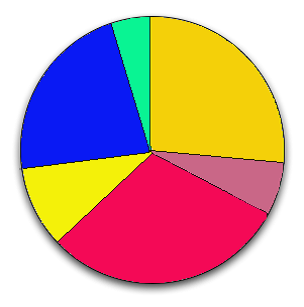
\includegraphics[width=0.3\textwidth]{figures/ruleta.png}
		\caption{Algoritmo de la Ruleta}
		\label{fig.ruleta}
		\end{center}
\end{figure}

Debajo de este modelo existen muchos parámetros relevantes para la implementación, de manera que entraremos un poco más en detalle: 
Se ha dicho que se debe disponer de un modelo de observación capaz de calcular las medidas láser de forma teórica de cada partícula y asociarles una probabilidad.

\begin{multicols}{2}
	\begin{figure}[H]
	\begin{center}
		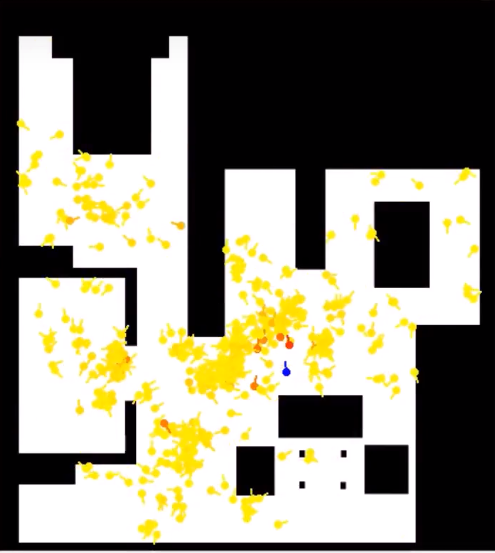
\includegraphics[width=0.4\textwidth]{figures/modeloobsv.png}
		\caption{Ejemplo de modelo de observación}
		\label{fig.modeloobsv}
		\end{center}
	\end{figure}
La Figura de la izquierda (\textbf{Figura 5.16}) muestra un ejemplo de este modelo, en el cual las partículas más lejanas a la posición del robot y en distinta orientación toman valores más bajos de probabilidad representados con un color más claro (amarillo), mientras que las cercanas a la posición real toman un valor más alto, representado en un color intenso (rojo). El cálculo del “láser teórico” es lo que permite asignar a cada una su probabilidad. Para obtenerlo, emplearemos un algoritmo de trazado de rayos sobre el mapa, que básicamente se basará en trazar
\end{multicols} una línea recta en el espacio bidimensional euclidiano desde la posición de cada partícula en la imagen hasta el punto donde se encuentre el máximo de distancia que puede abarcar el láser en las 9 direcciones que deben componer la lectura láser. En esta recta se va comprobando cada cierta distancia (paso $\lambda$) si el color del píxel es blanco (espacio libre) o negro(obstáculo), en cuyo caso se obtiene el punto en el que rebotaría el haz láser. Con ello, y conociendo la escala del mapa dado, obtenemos una distancia equivalente en la imagen para cada haz a la que se obtendría en el mundo si el robot ocupase esa posición. Así, 
\begin{equation}
X_{obstaculo} = (PX_{partícula} + \lambda*cos(\alpha_{haz}))*escala
\end{equation}
\begin{equation}
Y_{obstaculo} = (PY_{partícula} + \lambda*sin(\alpha_{haz}))*escala
\end{equation}
\begin{equation}
Distancia = \sqrt{(X_{obstaculo}-X_{partícula})^2+(Y_{obstaculo}-Y_{partícula})^2}
\end{equation}

Con esta distancia de cada haz, basta con compararla con la distancia que marca el sensor real en dicha orientación, con lo cual se obtendrá un error (error = LaserReal- LaserTeórico). Sólo es necesario acumular este error en cada orientación para asignar posteriormente una probabilidad. Cuanto menor error, las lecturas son más parecidas y se asignará la mayor probabilidad.

Por otro lado, el modelo de movimiento es de gran importancia para descartar información inservible y revalidar información adecuada. Se trata de incorporar el movimiento del robot a la generación de partículas en coordenadas polares $(\Delta r, \Delta\theta)$, para lo cual: 

\begin{equation}
\Delta x = x_{t+1} - x_{t}
\end{equation}
\begin{equation}
\Delta y = y_{t+1} - y_{t}
\end{equation}
\begin{equation}
\Delta\theta = \theta_{t} - \theta_{t-1}
\end{equation}
\begin{equation}
\Delta r = \sqrt{(\Delta x)^2+(\Delta y)^2}
\end{equation}

Bastará con sumar el incremento a la posición de cada partícula. Sin embargo, esta suma ha de ser consecuente con la orientación de la partícula (\textbf{Figura 5.17}), o más en concreto con el ángulo que forma ésta con respecto a la orientación del robot.

\begin{figure}[H]
\begin{center}
	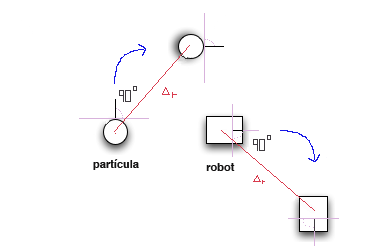
\includegraphics[width=0.4\textwidth]{figures/orientacionrelativa.png}
	\caption{Orientación Relativa}
	\label{fig.orientacionrelativa}
	\end{center}
\end{figure}

Hemos decidido aplicar geometría y trigonometría para poder materializarlo. En primer lugar, se construye una recta que pase por las coordenadas de la partícula $(x_{0},y_{0})$ a la cual se le va a sumar el movimiento. Esta recta se regirá por el vector de dirección creado a partir de la orientación de la partícula resultante al añadir el incremento angular:

\begin{equation}
a = cos(\theta_{0} + \Delta\theta)
\end{equation}
\begin{equation}
b = sin(\theta_{0} + \Delta\theta)
\end{equation}
\begin{equation}
y = y_{0} + \dfrac{b}{a} * (x-x_{0})
\end{equation}

Conociendo la distancia recorrida $(\Delta r)$, calculamos la coordenada x del nuevo punto al cual ha de desplazarse la partícula (y luego la coordenada y con la ecuación de la recta):

\begin{equation}
\Delta r = \sqrt{(x-x_{0})^2 + ((y_{0} + \dfrac{b}{a} * (x-x_{0}))-y_{0})^2} \Rightarrow x\, del\, nuevo\, punto
\end{equation}

Una vez hecho, ante un movimiento del robot, se tiene lo que se muestra en la \textbf{Figura 5.18}:

\begin{figure}[H]
\begin{center}
	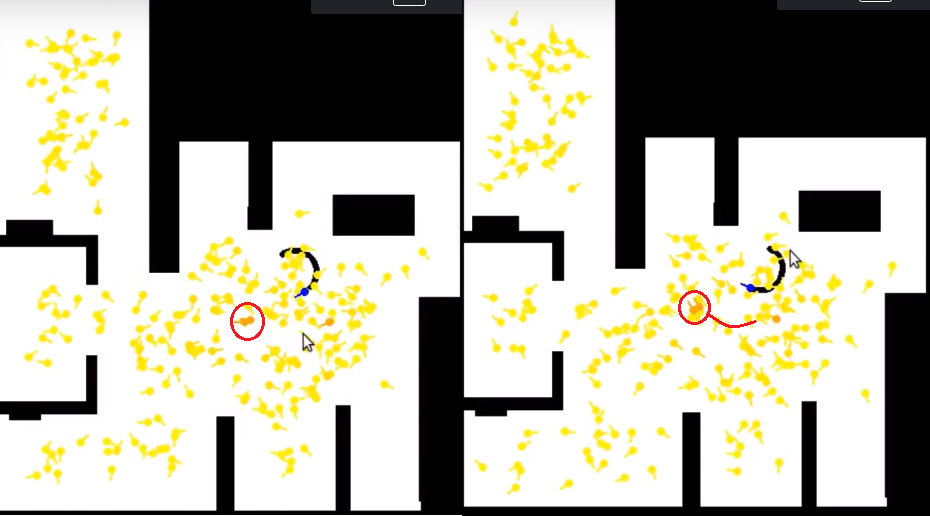
\includegraphics[width=0.65\textwidth]{figures/movimientoincorporado.png}
	\caption{Incorporación relativa de odometría}
	\label{fig.movimientoincorporado}
	\end{center}
\end{figure}

Por último, se ha de hacer hincapié en la forma de evolucionar hacia nuevas generaciones, de manera que estas acumulen cada vez mayor probabilidad y de esta forma converjan a la posición del robot. Ya se ha mencionado que se emplea el algoritmo de la ruleta. Para ello, se acumula la probabilidad de toda la generación $Pac(x_{i}) = P(x_{i})+Pac(x_{i-1})$, y luego se asocia a cada partícula un sector cuyo ancho es proporcional a la probabilidad individual de la partícula. El girar la ruleta se materializará a través de la obtención de un número aleatorio, el cual formará parte de un único sector dentro de la ruleta, saliendo a relucir la partícula que generará descendencia (\textbf{Figura 5.19}). La idea de este proceso es que las partículas que tienen alta probabilidad producen “picos” en la probabilidad acumulada, y por lo tanto tendrán más opciones de ser elegidas a la hora de muestrear. Así, una misma partícula puede tener muchos o hijos, o ninguno.

\begin{figure}[H]
\begin{center}
	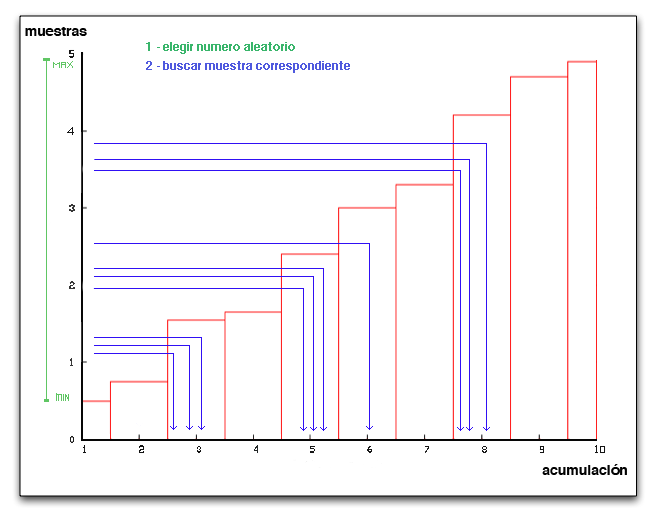
\includegraphics[width=0.65\textwidth]{figures/pacruleta.png}
	\caption{Algoritmo de la Ruleta y probabilidad}
	\label{fig.pacruleta}
	\end{center}
\end{figure}

Aunque en principio esta descendencia es idéntica a su progenitor, se puede evolucionar de manera más inteligente si se aplican algunas técnicas de selección, como el elitismo o el ruido térmico. Una vez seleccionado el progenitor, hemos decidido aplicar técnicas elitistas que persiguen conservar características de unas generaciones a otras de aquellas partículas de mayor probabilidad, distinguiendo y conservando la “élite” y eliminado las partículas que no aportan información. Así, si la partícula seleccionada para generar descendencia tiene una probabilidad muy superior a un umbral prestablecido, se copia en la siguiente generación, si su valor es ligeramente superior al umbral, se aplica un ruido térmico (gaussiano) de posición y orientación centrado en el progenitor para generar el hijo y si no supera el umbral se lanza una nueva partícula aleatoria, como al inicio del algoritmo. Esto permite conservar la información relevante, eliminar la inútil y lo más importante: permite explorar los alrededores de las partículas que acumulan mayor probabilidad, pudiendo así encontrar partículas de mayor calidad en cada generación. Esto también aplica en el cálculo de la probabilidad acumulada, ya que si ésta no supera un umbral, se considera que no aporta información y se descarta la generación entera, remuestreando con una nueva generación aleatoria.

Hay diferentes modos de implementación de lo anterior en función de la aplicación que se quiere construir. En los siguientes apartados se desarrollará las características de implementación que se han seguido en este caso.

\subsection{Métodos de optimización}
Aún con la reducción de puntos del espacio posibles que acompañan al filtro de partículas, queda de manifiesto que se necesita cubrir gran parte del espacio dado para obtener valores representativos del mismo. Por ello, se ha decidido utilizar 650 partículas distribuidas por la escena, para cada una de las cuales se debe calcular 9 haces láser teóricos para asociarles una probabilidad, procesando en cada una la imagen del mapa en función de su posición. Es por eso que para aplicaciones en tiempo real (como es el caso) empieza a ser crítico el intervalo empleado en la computación, sobre todo si se trata de robot en movimiento. 

Algunas decisiones tomadas en la implementación y mencionadas en apartados anteriores se explican a través de la necesidad de lograr un algoritmo ágil y eficiente. Por ejemplo, el hecho de haber utilizado 9 haces por láser en lugar de los 180 disponibles se debe a que este número de haces es suficiente para obtener lecturas representativas del entorno en cualquier punto, de manera que todos los otros rayos sólo aportarán en casos muy extremos, pero generalmente ralentizarán en gran medida el comportamiento del algoritmo y reducirán al mínimo su eficiencia. 
También el hecho de segmentar la funcionalidad de la práctica en distintos hilos de ejecución se debe a esto, ya que existían distintas tareas que se podían realizar de manera concurrente y compatible, ya que ninguna de ellas se cruza con las demás (toma de datos de sensores, interfaz y algoritmo).
Por otro lado, ya en términos de código, se ha decido precomputar todos los datos posibles para aumentar la eficiencia al máximo en cada iteración.

\subsection{Solución desarrollada}
Con todo lo anterior, la secuencia utilizada para organizar la lógica es:
En primer lugar, si no se ha establecido generación de partículas se utiliza el método \textit{sendParticles()} para establecerlas de la manera aleatoria inicial. Este método se encarga de todo lo necesario para obtener una primera generación, incluyendo el trazado de rayos de cada partícula para la obtención de su láser teórico con \textit{doRayTracing()} y con él la probabilidad a través de \textit{calculateProb()}. Hay involucradas otras funciones que comprueban si el color de un pixel es blanco o negro (\textit{isWhitePixel}), que realizan el parsing de la información láser (\textit{parse\_laser\_data()}) y otras como el método \textit{uniform} de la biblioteca random para obtener las posiciones aleatorias entre otras. Lo siguiente es la incorporación de la odometría a través del modelo de movimiento, donde se actualizan todas las partículas y se gestiona si el movimiento incorporado invalida alguna partícula (tras el movimiento, algunas partículas pueden quedar fuera de los límites del espacio libre), en cuyo caso se genera una nueva partícula aleatoria. Esta incorporación es relativa a la posición y orientación de cada partícula. A través del API de posición descrito en \textbf{5.3} se accede fácilmente a dicha información. En este punto tendremos algo similar a la \textbf{Figura 5.20}:

\begin{figure}[H]
\begin{center}
	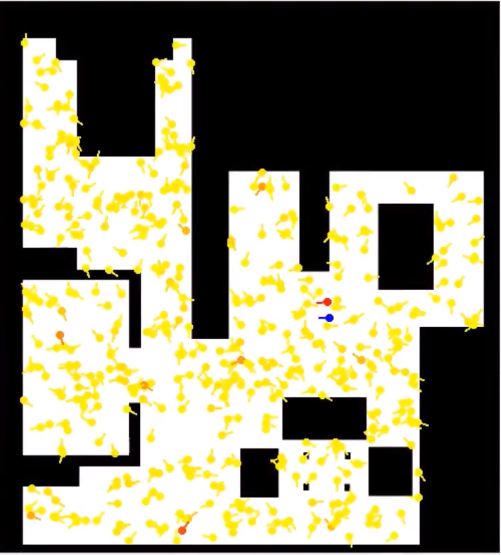
\includegraphics[width=0.45\textwidth]{figures/primerageneracion.png}
	\caption{Primera generación de partículas}
	\label{fig.primerageneracion}
	\end{center}
\end{figure}  

Tras esto, es el momento de evolucionar a nuevas generaciones, si procede (con \textit{calculateNewGeneration()}). En todas las iteraciones no se realiza el cálculo de nuevas generaciones, ya que esto consume toda la capacidad del procesador. En base a distintas pruebas realizadas, hemos decidido implementar un reloj de generación, que evolucionará generaciones cada 300ms.
Si se trata de una iteración de generación, los siguientes pasos son:

\begin{itemize}
	\item[--] Comprobar si la generación converge. Para ello seleccionamos la partícula de mayor probabilidad de la generación y calculamos la distancia euclidiana entre esta y cada una de las otras partículas. Si todas ellas se encuentras comprendidas en una circunferencia de radio 2m, se considera que la generación converge, y es hora de hacer una estimación con la partícula de mayor probabilidad.
	\item[--] En caso de no convergencia, y teniendo en cuenta las técnicas elitistas, en cada nueva generación se comprueba si la partícula más probable supera el 99\% de coincidencia, en cuyo caso también hemos decidido hacer una estimación de posición.
	\item[--] En el resto de casos se calcula una nueva generación a partir de la anterior, calculando en primer lugar la probabilidad acumulada como la suma de todas las probabilidades, luego ejecutando el algoritmo de la ruleta una vez por cada nueva partícula que se quiera generar, en nuestro caso 650 veces, y con la partícula seleccionada se haga el filtro de partícula correspondiente (a través de \textit{particlesFilter}).
	\item[--] Este filtro aplicará las técnicas de selección, el ruido gaussiano y el remuestreo cuando proceda, en función de la salud de la partícula.
	\item[--] En todo caso, tras una estimación se crea una nueva generación aleatoria.
	\item[--] Habrá iteraciones de generación en las que no se haga ninguna estimación
	\item[--] Hay condiciones de parada, como un número máximo de iteraciones de generación sin estimación, para descartar datos que no llevan a una estimación correcta. 
\end{itemize}

A parte de esto, el algoritmo propuesto se encarga de establecer las estimaciones para que sean visibles en la interfaz, y también de gestionar el cálculo de un láser concreto cuando se hace click sobre una partícula del mapa, para poder mostrarlo en el \textit{widget} de representación láser.

La solución planteada incorpora todo lo anterior, pasando por un proceso de ajuste de cada módulo de manera independiente. Para ajustar el modelo de observación láser empleado, y que las probabilidades que asigne se adecúen a la escena, se han usado distintos métodos:
\vspace{4cm}

\textbf{Malla de partículas}

\begin{multicols}{2}
	\begin{figure}[H]
		\begin{center}
		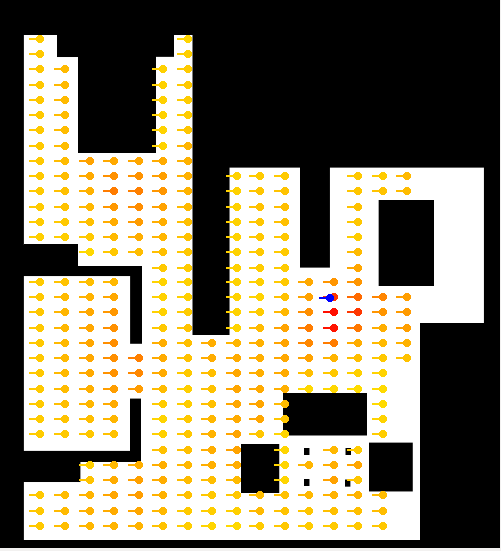
\includegraphics[width=0.45\textwidth]{figures/mallaparticulas.png}
		\caption{Malla de partículas}
		\label{fig.mallaparticulas}
		\end{center}
	\end{figure}
Se trata de crear una especie de rejilla de partículas (\textbf{Figura 5.21}), de manera que se puede ver de forma gráfica y sencilla la distribución de la probabilidad. Para partículas cercanas al robot, las representaciones asociadas deben tomar un color más rojo, mientras que las lejanas deben tirar más hacia el amarillo. Jugando con la separación entre partículas obtuvimos la función del modelo de observación idónea para el tipo de comparación implementado entre el láser real y el teórico.
\end{multicols}

\textbf{Slider de Orientación de partículas}

\begin{multicols}{2}
De manera análoga a lo anterior, se incluyó un slider (\textbf{Figura 5.22}) que permitía controlar la orientación de todas las partículas al unísono y recalcular su probabilidad tras el cambio, lo cual permitió ajustar 
	\begin{figure}[H]
		\begin{center}
		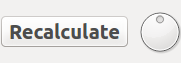
\includegraphics[width=0.30\textwidth]{figures/slider.png}
		\caption{Slider de orientación}
		\label{fig.slider}
		\end{center}
	\end{figure}
\end{multicols}
en mayor medida el modelo de observación, ya que partículas en posición cercana y orientación similar (con variaciones entre 0º y 10º) deben tener una probabilidad alta, pero en posiciones similares y orientaciones distintas (>20º) deben tener probabilidades bajas (\textbf{Figura 5.23}).

\begin{figure}[H]
		\begin{center}
		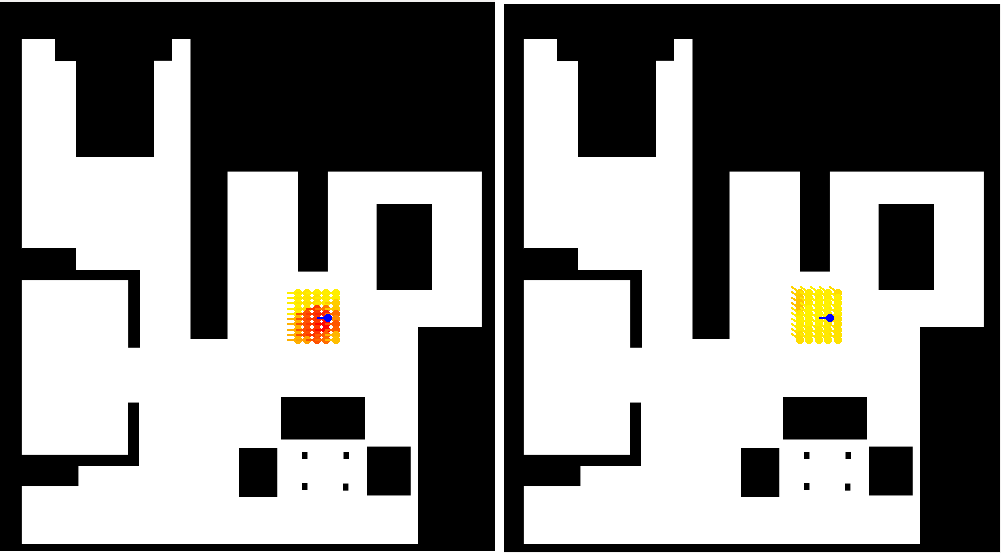
\includegraphics[width=0.85\textwidth]{figures/slidermap.png}
		\caption{Ajuste de Modelo de Observación (diferencia angular de 0º vs. diferencia angular de 40º)}
		\label{fig.slidermap}
		\end{center}
	\end{figure}
	
\textbf{Ruido Gaussiano}
	
Para llevar a cabo la exploración de una zona en la que existe una partícula de alta probabilidad, pero insuficiente para hacer una estimación, la descendencia de la misma se crea añadiendo un pequeño ruido que no debe dispersar demasiado las nuevas partículas generadas, ya que la intención es encontrar una nueva posición más favorable, la cual tiene altas probabilidades de estar muy cerca y en una orientación muy parecida. Se probó con diferentes configuraciones de ruido, para al final decantarnos por una distribución normal centrada en la posición del progenitor con una desviación típica $\sigma$ de 0.1.

Aunque estos son los ajustes más importantes, hicieron falta otros que han influido en el rendimiento del algoritmo final, los cuales se comentarán en los siguientes puntos.

\section{Experimentación}
En este apartado demostraremos que la funcionalidad descrita en los apartados anteriores ha sido incluida en el algoritmo a través de experimentos realizados para poner a prueba cada una de las partes, así como la infraestructura de la práctica y el nodo.

\subsection{Ejecución típica}
Se ha preparado un documento de texto plano (\textit{README.md}) que sirve de guía para que alumno este guiado durante la ejecución y el testeo, que incluye también información del API de utilización, e incluso una referencia a un vídeo demostrativo. 

La forma de ejecutar la práctica basada en interfaces de ROS, la cual establecemos como definitiva, es la siguiente:

\begin{enumerate}
	\item 1.	Empleamos un primer terminal para ejecutar el componente que lanza un mundo Gazebo basado en componentes de ROS:
	\begin{figure}[H]
		\begin{center}
			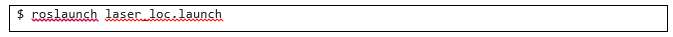
\includegraphics[width=0.95\linewidth]{figures/llcomando1.png}
			\label{fig.llcomando1}
		\end{center}
	\end{figure}
	\item 2.	Utilizamos un segundo terminal para iniciar el componente académico:
	\begin{figure}[H]
		\begin{center}
			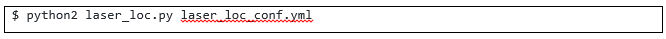
\includegraphics[width=0.95\linewidth]{figures/llcomando2.png}
			\label{fig.llcomando2}
		\end{center}
	\end{figure}
\end{enumerate}

Pulsando sobre el botón “Play Code” se podrá ver el resultado de la ejecución del algoritmo, el cual una vez escrito producirá una salida como la siguiente:

Ejemplos de la ejecución pueden encontrarse en:
 
\url{https://www.youtube.com/watch?v=FmUN_tzM9MM} , y

\url{https://www.youtube.com/watch?v=4OFljaeag_I}

A continuación, una serie de capturas de una ejecución (\textbf{Figura 5.24}),

\begin{figure}[H]
	\begin{center}
		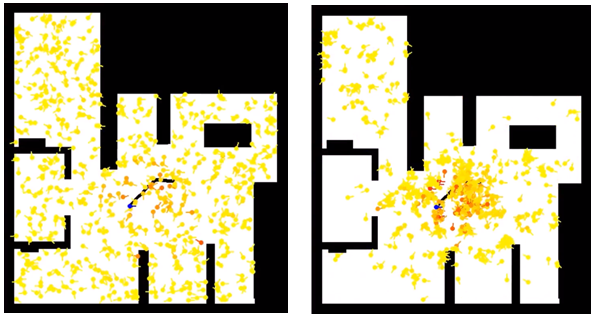
\includegraphics[width=0.850\textwidth]{figures/lloutput1.png}
		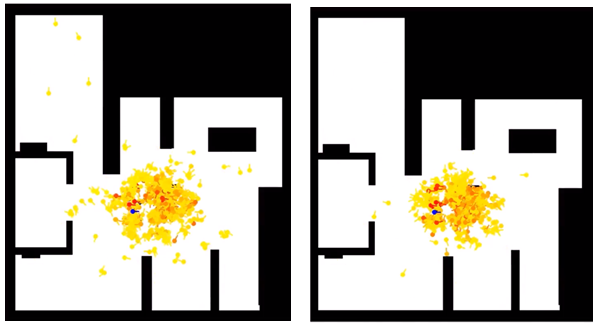
\includegraphics[width=0.850\textwidth]{figures/lloutput2.png}
		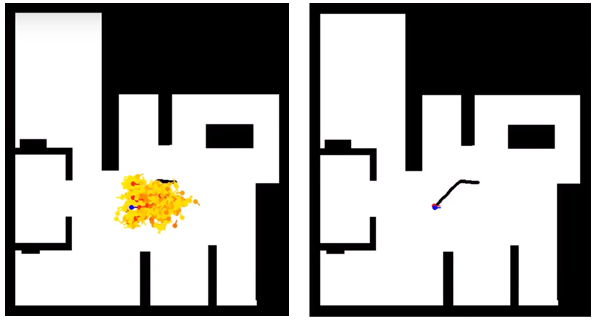
\includegraphics[width=0.850\textwidth]{figures/lloutput3.png}
		\caption{Output Laser Loc}
		\label{fig.outputll}
		\end{center}
\end{figure}

\subsection{Ajuste del tiempo de evolución de las partículas}
Ya se ha mencionado que las generaciones no se evolucionan en todas las iteraciones del algoritmo, sino que se ha establecido un tiempo de evolución. El ajuste de este tiempo se basado en la rapidez del algoritmo en proporcionar una estimación: de media han sido necesarias 13 generaciones para obtener una estimación, y en vistas a lograr la localización de un robot en movimiento, se decidió que era necesaria al menos 1 estimación cada 4 segundos, de manera que se fijó dicha evolución en intervalos de 300 ms. 

\subsection{Localización en movimiento}
Además del evidente problema de que un robot no estático implica tener partículas no estáticas, también se debe pensar en el número de eventos que el movimiento del robot genera en el nodo. Al moverse el robot, no sólo se debe gestionar la comunicación con sus interfaces, sino que también se envían órdenes al interfaz para el teleoperador, para repintar el robot en el mapa, para actualizar la trayectoria y para añadir el modelo de movimiento a las partículas. Gracias al tiempo de evolución y a la programación multihilo esto es posible de manera simultánea.

Hay que darse cuenta de que el robot debe estimar su posición el mayor número de veces posible en el menor intervalo de tiempo, ya que de otro modo podría provocar un malfuncionamiento en alguna otra tarea del robot al no haber completado su localización (normalmente los algoritmos de localización se usan en conjunción con algoritmos controladores que desempeñan otras tareas para las cuales se hace necesario conocer la posición actual). Debido a esto, la localización con movimiento implicado es una manera de poner a prueba el algoritmo en un caso complejo.

Salvando fallos iniciales en algunas ejecuciones (estimaciones erróneas por algunos metros en las primeras iteraciones, pero tolerables al principio de la ejecución), los errores de posición estimada obtenidos no superan en ningún caso los 20cm desde el centro del robot, siendo la media de menos de 10cm (\textbf{Figura 5.25}):

\begin{figure}[H]
	\begin{center}
		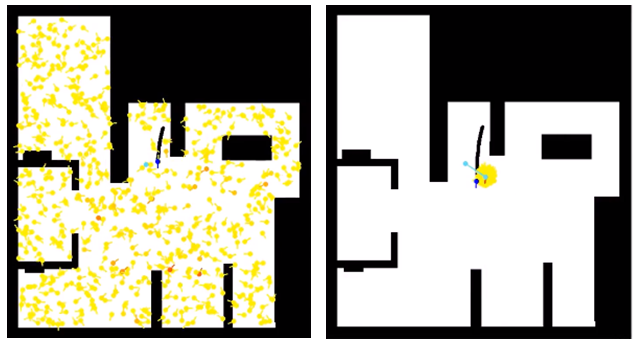
\includegraphics[width=0.850\textwidth]{figures/lloutputmov1.png}
		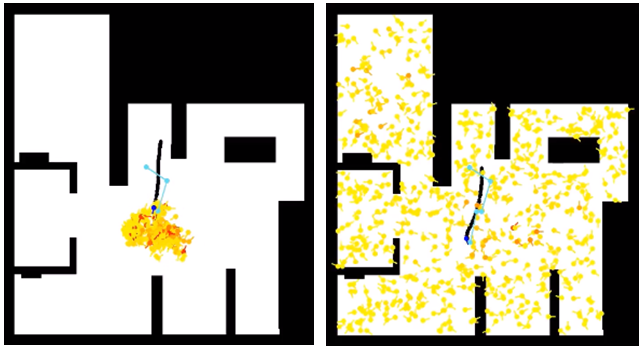
\includegraphics[width=0.850\textwidth]{figures/lloutputmov2.png}
		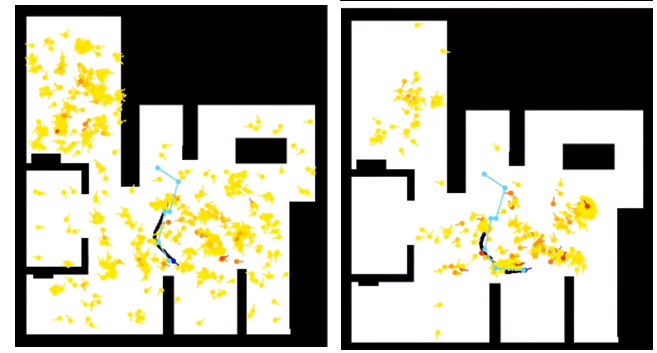
\includegraphics[width=0.850\textwidth]{figures/lloutputmov3.png}
		\caption{Output Laser Loc en movimiento}
		\label{fig.outputllmov}
		\end{center}
\end{figure}

\subsection{Comportamiento ante casos extremos}
Llegados a este punto y comprobado el funcionamiento del algoritmo, decidimos ponerlo a prueba en condiciones complejas, para comprobar si la solución propuesta era lo suficientemente buena como para lidiar con los problemas que podían surgir en entornos reales.

Aunque los escenarios simulados están compuestos por elementos de distinta naturaleza, en muchas ocasiones se tienen espacios concretos con una geometría similar (\textbf{Figura 5.26}), que para el ojo humano es claramente distinguible, pero no así a priori para los sensores que puede incorporar un robot. Decidimos localizar dichos puntos en nuestro mundo, y comprobar que ocurría:

\begin{multicols}{2}
\begin{figure}[H]
	\begin{center}
		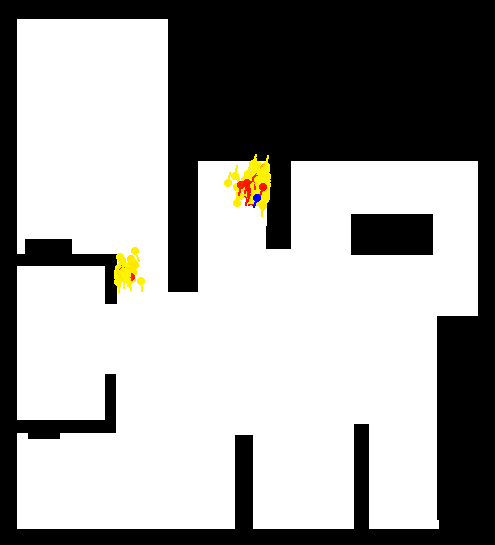
\includegraphics[width=0.49\textwidth, height=10.5cm]{figures/similar.png}
		\caption{Espacios de geometría similar}
		\label{fig.similar}
		\end{center}
\end{figure}
Tras unas cuantas iteraciones, se forman una serie de frentes de partículas que acumulan una probabilidad similar (tantos como lugares con geometría parecida existan en el entorno). Antes casos como este, el algoritmo de localización necesitó bastantes más iteraciones de evolución de generaciones (al menos el doble en la mayoría de los casos), pero en el 70\% de ellos la estimación final venía del grupo situado en la posición correcta, es decir, en los alrededores del robot (\textbf{Figura 5.27}).
\begin{figure}[H]
	\begin{center}
		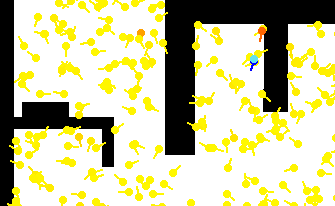
\includegraphics[width=0.38\textwidth, height=2.5cm]{figures/similaroutput.png}
		\caption{Output en espacios similares}
		\label{fig.similaroutput}
		\end{center}
\end{figure}
\end{multicols}

Normalmente, los problemas en el resto de casos se solucionan añadiendo algún otro sensor que ayude a descartar unos datos frente a otros, o simplemente incorporando movimiento, pues las posibles similitudes se irán desvaneciendo a medida que el robot avance.

Por otro lado, y en relación con el experimento anterior, decidimos ver que sucedía en caso de situar al robot muy cerca de las superficies límite (de los obstáculos).

\begin{figure}[H]
	\begin{center}
		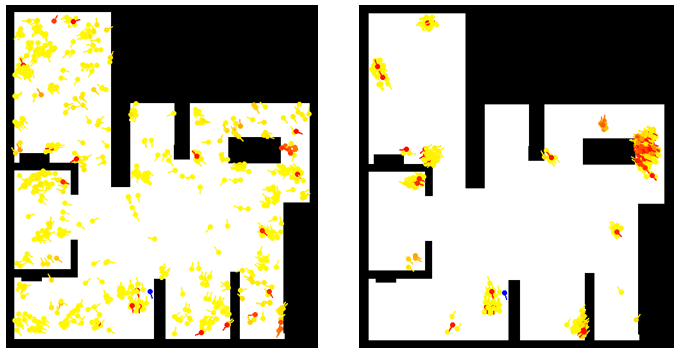
\includegraphics[width=0.88\textwidth]{figures/estampado.png}
		\caption{Posición cercana a los obstáculos}
		\label{fig.estampado}
		\end{center}
\end{figure}

En estos casos (\textbf{Figura 5.28}), el robot obtiene muchos puntos en los que podría obtener una lectura dentro de los márgenes de similitud con la lectura real, de manera que se generan muchos \textit{clusters} de partículas, que pueden evolucionar favorablemente o no, dependiendo de cómo fuese la distribución aleatoria inicial (recordemos que las sucesivas generaciones surgen siempre de alguna partícula preexistente). Este experimento confirmó que un algoritmo de localización robusto debe valerse de datos de distintos sensores: puede basarse en láser pero necesita incorporar por ejemplo información de textura para lidiar con esto

Por último, sabiendo que en la realidad se dan muchos espacios simétricos (salas cuadradas, mobiliario rectangular,…), quisimos hacer un experimento en un entorno altamente simétrico, para lo cual sirvió el modelo explicado en \textbf{5.2.3}, el cual es cuadrado y sólo incorpora algunos elementos que pueden generar lecturas distintas en algunos puntos. Además, sirvió para demostrar la compatibilidad del nodo y de la práctica en general con distintos mundos simulados (\textbf{Figura 5.29}):

\begin{figure}[H]
	\begin{center}
		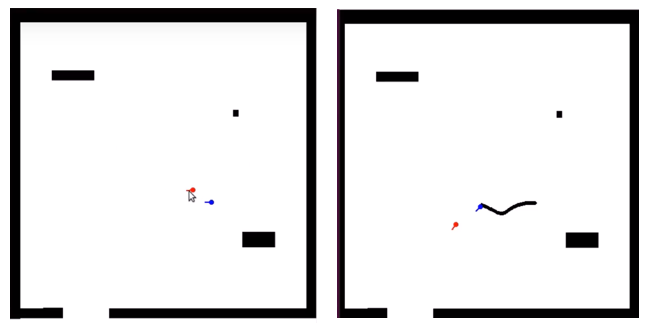
\includegraphics[width=0.88\textwidth]{figures/outputsimetrico.png}
		\caption{Output en entorno simétrico}
		\label{fig.outputsimetrico}
		\end{center}
\end{figure}

El algoritmo continuó funcionando y realizando estimaciones de posición, aunque éstas en muchos casos empezaban a obtener errores más elevados, en torno a los 10-15 cm. En muchas ocasiones, estos errores pueden verse incrementados por el error que se haya cometido en el modelado del mapa, pero en cualquier caso el factor más influyente es la simetría, que al ser notable puede traducirse en distintos puntos de la sala con lecturas muy poco cambiantes. De nuevo, el hecho de la generación inicial aleatoria influirá en el error cometido, ya que no se coloca una partícula por cada punto posible (en cuyo caso siempre obtendríamos una localización exacta), y por tanto la localización varía aunque se trate del mismo punto en distintas ejecuciones.

\section{Laser\_Loc a través de Jupyter}
Tras comprobar de primera mano las grandes ventajas que tiene Jupyter y la potencia de la que dispone para ejecutar nuestras aplicaciones de escritorio vía web, y después de haber resuelto una versión del nodo académico a través de ROS para la práctica de autolocalización, decidimos combinar ambas cosas para ampliar en gran medida el espectro de usuarios que pueden acceder a la práctica, y enfrentarse a ella con éxito. Una vez hecha una versión a través de Jupyter, tendremos una práctica totalmente auto-contenida (independiente del paquete de comunicaciones de JdeRobot) y basada en \textit{ROS Messages}, lo cual se traduce en un mayor número de usuarios potenciales, ya que está disponible en multitud de plataformas. Sabemos que las tecnologías web sólo dependen del cliente utilizado (no así de la plataforma), de manera que futuros estudiantes de JdeRobot-Academy sólo tendrán que instalar el simulador, las bibliotecas necesarias de \textit{ROS Kinetic} y un pequeño paquete de JdeRobot con los mundos y modelos del simulador.

Sin embargo, esta práctica lleva mucha más carga y complejidad gráfica de la que llevaba la descrita en el \textbf{Capítulo 4}, de manera que hemos tenido que explorar las opciones de interfaz que ofrece esta herramienta. Aunque ésta permite lanzar subprocesos desde los \textit{Notebooks}, la idea que nos ha resultado más atractiva ha sido la de construir \textit{widgets} interactivos, controlados por código Python, a través de bibliotecas de representación como \textit{MatPlotLib}, que recogen eventos de usuario y los materializan en la funcionalidad necesaria, permitiendo así disponer de una interfaz gráfica en el cuadernillo. Con estos nuevos integrantes sumados a los que ya habíamos empleado (celdillas de código, imágenes, texto con formato, etc.) hemos preparado un Notebook de Jupyter al que hemos llamado \textit{laser\_loc.ipynb} (\textbf{Figura 5.30}), a través del cual accederemos a la versión de Jupyter de esta práctica. En esta ocasión, los cambios en el nodo son más notables, dado que es necesario gestionar toda la funcionalidad de interacción desde el mismo, y además construir la forma de comunicación entre éste y el \textit{kernel} de Jupyter. En concreto, el nodo programado en el fichero \textit{lase\_loc.py} de la práctica original ha sido recodificado para tener estructura de clase Python (\textit{LaserLoc}), a la cual le hemos incorporado todos los atributos y métodos necesarios tanto para el soporte de la práctica como para su parte gráfica. 

\begin{figure}[H]
	\begin{center}
		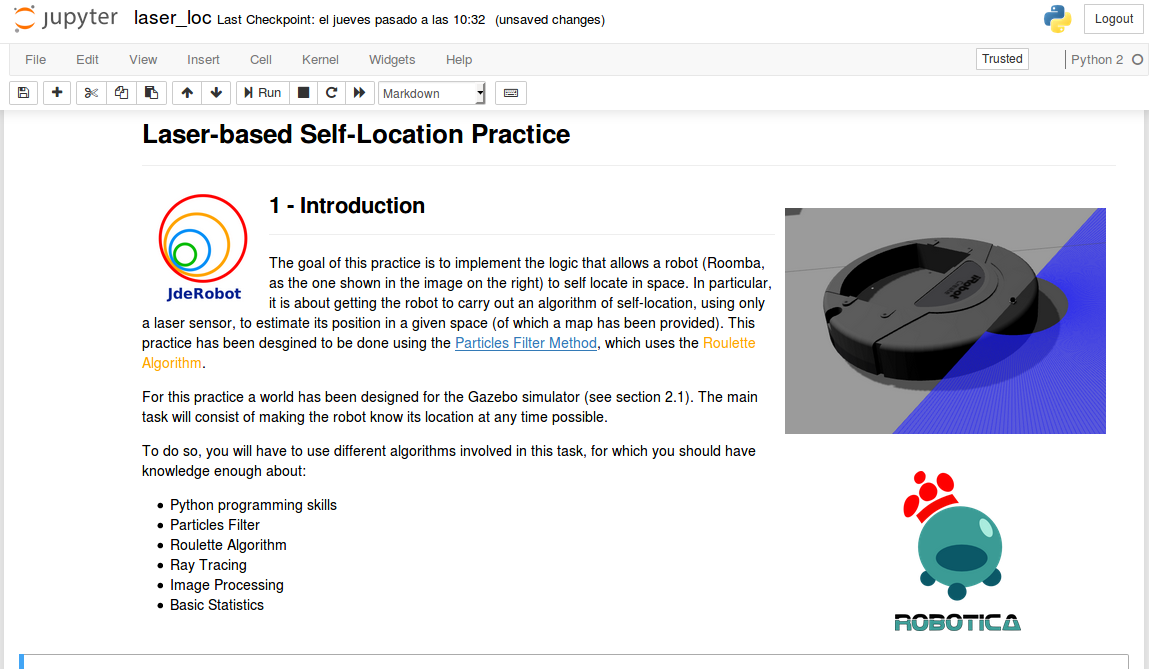
\includegraphics[width=0.98\textwidth]{figures/laserlocjupyter.png}
		\caption{Notebook de LaserLoc}
		\label{fig.laserlocjupyter}
		\end{center}
\end{figure}

Aunque los elementos principales del \textit{Notebook} son los \textit{widgets} interactivos y las celdas de código, también se ha incluido texto de apoyo para los pasos a seguir en la resolución de la práctica e imágenes representativas de las salidas que se pueden ir obteniendo, todo lo cual creemos que es de gran ayuda para orientar al alumno, en especial, la descripción del API de funcionalidad que la clase \textit{LaserLoc} del cuadernillo pone a su disposición.

En cuanto a los elementos interactivos, hemos decidido incluir principalmente dos dinámicos y uno estático basados en los que ya había en la interfaz de la versión de escritorio de la práctica:

\textit{Teleoperador}

\begin{figure}[H]
	\begin{center}
		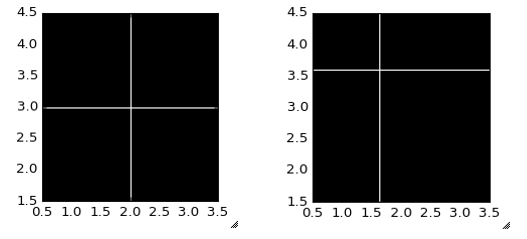
\includegraphics[width=0.68\textwidth]{figures/teleoperadorjupyter.png}
		\caption{Teleoperador en Jupyter}
		\label{fig.laserlocjupyter}
		\end{center}
\end{figure}
Este controlador (\textbf{Figura 5.31}) no es más que una representación básica de dos rectas sobre un fondo negro. Sin embargo, ha sido preparado para recoger eventos del ratón desde la aplicación (\textit{press} y \textit{release}), y para enviar órdenes a los actuadores del robot en función de estos y que se reflejen en la simulación. Así, si el usuario hace click sobre este \textit{widget}, arrastra la cruz hasta un punto determinado y deja de presionar el ratón, consigue materializar un movimiento proporcional al movimiento de la cruz en el robot. Con este elemento mantenemos la posibilidad de probar el algoritmo en condiciones de localización en movimiento.

\textit{Mapa Binario}

\begin{figure}[H]
	\begin{center}
		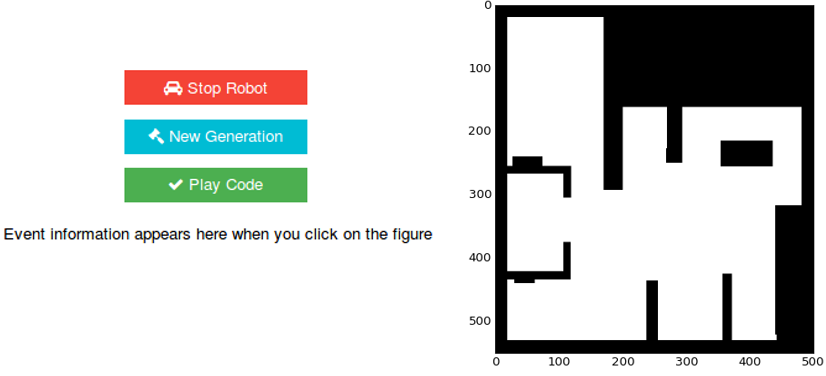
\includegraphics[width=0.90\textwidth]{figures/mapabinariojupyter.png}
		\caption{Widget de Mapa Binario en Jupyter}
		\label{fig.mapabinariojupyter}
	\end{center}
\end{figure}
Este \textit{widget} (\textbf{Figura 5.32}) consta de varios elementos. Como se puede ver en la Figura superior, se han dispuesto 3 botones que también recogen interacción. El primero (en rojo), tiene que ver con el \textit{widget} anterior, y sirve para parar el movimiento del robot y restablecer la posición del teleoperador, para facilitar el control del mismo. El segundo (en azul) es el que se utiliza para ejecutar la función \textit{cretaeNewGeneration}, una de las dos que el alumno debe implementar para alcanzar la solución. Esta función es la encargada de evolucionar las generaciones bajo la orden del alumno, el cual genera un nuevo conjunto de partículas basado en el precedente con cada click. Por último (en verde), el botón \textit{Play Cod}e ejecuta el código del método \textit{execute}, el cual también debe ser codificado por el alumno, que recoge la funcionalidad principal del algoritmo, y que debe gestionar también el cálculo del láser de una posible partícula sobre la que se haga click en el mapa.

El elemento principal del \textit{widget} es el mapa, que se ha extrapolado directamente desde la interfaz de la práctica, siendo una imagen binaria que permitirá visualizar la evolución del algoritmo. También es un elemento dinámico, que variará cada vez que se evolucione una generación, y que recogerá los clicks del usuario para traducir las coordenadas del ratón en coordenadas de una partícula y así poder realizar el cálculo de su láser y su representación.

\textit{Representación láser}

\begin{multicols}{2}
\begin{figure}[H]
	\begin{center}
		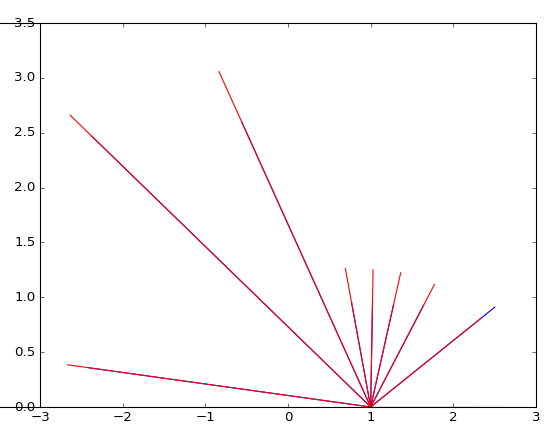
\includegraphics[width=0.49\textwidth]{figures/laserjupyter.png}
		\caption{Widget Láser en Jupyter}
		\label{fig.laserjupyter}
	\end{center}
\end{figure}

Este \textit{widget} (\textbf{Figura 5.33}) estático es equivalente a la gráfica de los láseres real y teórico de la práctica original. En cuanto se hace click sobre una partícula en el mapa, si se ejecuta la celdilla de código del \textit{Notebook} indicada para la representación láser, se tendrá algo como lo que se muestra en la Figura de la izquierda, donde el láser teórico (rojo) se superpone a los datos reales (azul). La celdilla de este elemento también mostrará por su salida la probabilidad asociada a la partícula sobre la que se ha hecho click.
\end{multicols}

Todos estos elementos contribuyen a que la funcionalidad de la práctica esté soportada desde Jupyter, de manera que en una ejecución concreta se obtienen outputs equivalentes a los que se obtendrían fuera de esta aplicación:

\begin{figure}[H]
	\begin{center}
		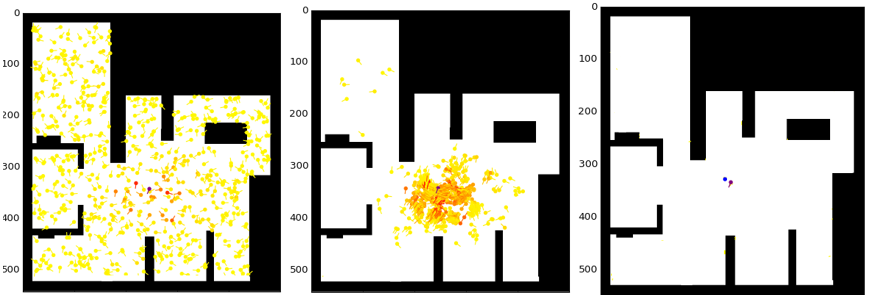
\includegraphics[width=0.99\textwidth]{figures/outputjupyterll.png}
		\caption{Output de LaserLoc en Jupyter}
		\label{fig.laserjupyter}
	\end{center}
\end{figure}

Un vídeo demostrando el comportamiento de la práctica a través de Jupyter se puede ver en:

\url{https://www.youtube.com/watch?v=kF7szwrC6a0}
